\documentclass[a4paper, twoside]{article}
\usepackage[utf8]{inputenc} % Especifica la codificación de caracteres de los documentos.
\usepackage[spanish]{babel} % Indica que el documento se escribirá en español.
\usepackage[top=3cm, bottom=2.5cm, inner=1.5cm, outer=2.5cm]{geometry} % Márgenes personalizados
\usepackage{subfiles} % Paquete para incluir el preambulo en los sub archivos.
\usepackage{afterpage} % Permite añadir páginas despues de una página dada.
\usepackage{hyperref} % Permite incluir enlaces en los archivos.
\usepackage{lastpage} % Paquete para poder contabilizar el total de páginas del documento.
\usepackage{fancyhdr} % Permite personalizar los header y footer del documento.
\usepackage{graphicx} % Permite incluir gráficos
\usepackage[hang, bf]{caption} % Personaliza los subtítulos de las figuras y tablas
\usepackage{float} % Permite posicionar mejor las figuras y tablas
\usepackage{listings} % Permite insertar código fuente
\usepackage{xcolor} % Permite utilizar más colores.

\definecolor{darkblue}{rgb}{0,0,0.4}
\definecolor{darkgreen}{rgb}{0,0.4,0}

% Defino la ruta de los paquetes personalizados para el apunte
\newcommand{\rutapaquetes}{./paquetes-apunte}

\usepackage[mostrarlicencia]{\rutapaquetes/caratula} % Caratula personalizada (cargada desde caratula.sty)
\usepackage[ocultarrevisores]{\rutapaquetes/colaboradores} % Seccion de colaboradores (cargada y creada con colaboradores.sty)
\usepackage{\rutapaquetes/historial} % Seccion de historial de cambios (cargada y creada con historial.sty)

% Define los estilos de los enlaces interpretados por el paquete hyperref
\hypersetup{
	colorlinks=true,   % false: boxed links; true: colored links
	linkcolor=black,   % color of internal links (change box color with linkbordercolor)
	citecolor=green,   % color of links to bibliography
	filecolor=magenta, % color of file links
	urlcolor=blue     % color of external links
}

\newcommand{\imgdir}{../resources/images} % Ruta de las imágenes

% Define los directorios de las imágenes y gráficos
\graphicspath{ {\imgdir/} {\rutapaquetes/} }

\newcommand{\nombremateria}{Sistemas Operativos (75.08 - 95.03)} % Defino el comando "\nombremateria" para no harcodear el nombre en varios lugares.

% Define el pagestyle personalizado
\pagestyle{fancy}
\fancyhf{}
\renewcommand{\sectionmark}[1]{\markboth{}{\thesection\ \ #1}}
% Define header para pagina par
\fancyhead[ER]{\rightmark}
% Define header para pagina impar
\fancyhead[OL]{\rightmark}
% Define footer para pagina par
\fancyfoot[EL]{\nombremateria} % Nombre del apunte a la izquierda
\fancyfoot[ER]{Página \thepage\ de \pageref{LastPage}} % Numero de pagina a la derecha
% Define footer para pagina impar
\fancyfoot[OL]{Página \thepage\ de \pageref{LastPage}} % Numero de pagina a la izquierda
\fancyfoot[OR]{\nombremateria} % Nombre del apunte a la derecha

\renewcommand{\footrulewidth}{0.4pt} % Agrego linea que separa el footer

% Elijo formato de bloques de código fuente
\lstset{ 
	backgroundcolor=\color{white},
	basicstyle=\ttfamily\footnotesize,
	breaklines=true,
	commentstyle=\color{darkgreen},
	extendedchars=true,
	frame=single,
	language=C++,
	literate={á}{{\'a}}1 {é}{{\'e}}1 {í}{{\'i}}1 {ó}{{\'o}}1 {ú}{{\'u}}1 {ñ}{{\~n}}1, % Escapeo caracteres especiales
	keywordstyle=\color{darkblue},
	numbers=left,
	numberstyle=\tiny\color{gray},
	tabsize=4,
	showspaces=false,
	showstringspaces=false,
	stringstyle=\color{red}
}

% Configura la caratula
\materia{\nombremateria}
\tipoapunte{Resumen teórico}
%\tema{Tema de la Materia}
%\subtema{Subtema}

\begin{document}
% Página en blanco agregada después de la carátula
%\afterpage{
%	\null
%	\thispagestyle{empty}%
%	\addtocounter{page}{-1}%
%	\newpage}
\maketitle % Genera la carátula

\tableofcontents % Genera el índice

\subfile{\rutapaquetes/acerca-del-proyecto.tex} % Incluye información acerca del proyecto FIUBA Apuntes

\section{Introducción}
\subsection{¿Qué es un sistema operativo?}
\begin{itemize}
	\item Un programa que hace de intermediario entre el usuario de la computadora y su hardware (Oculta los detalles finos de la arquitectura).
	\item Un programa que administra los recursos de un sistema de computación: permite administrar el tiempo de procesador y el espacio (memoria, disco, etc).
\end{itemize}

\subsection{Arquitecturas}
\subsubsection{Mainframe}
Computadora central. Gran capacidad de I/O, server para e-commerce a gran escala.\\

\textbf{Seguridad y disponibilidad:} 
\begin{itemize}
	\item Transaction processing: es procesamiento de información distribuido en operaciones individuales e indivisibles, llamadas \emph{transacciones}. Cada transacción debe ser exitosa o fallar como unidad entera, no puede haber transacciones parcialmente completas.
	\item Batch processing: Es la ejecución de una serie de programas ("tareas") en una computadora sin intervención del usuario.
\end{itemize}

\subsubsection{Servidores}
Destinados a ofrecer servicios a través de una red.

\subsubsection{Supercomputadoras}
Computación de alto rendimiento. Se usan para hacer simulaciones.\\

\textbf{Limites:}
\begin{itemize}
	\item Concurrencia: los procesos no son 100\% independientes
	\item Costo
	\item Programación del software
\end{itemize}

\subsubsection{Server operating system}
Interfaz solo línea de comando o EFI (estándar de firmware).

\subsubsection{Computadora personal}
No requiere conocimientos especiales.

\subsubsection{Tablets, PDA}

\subsubsection{Consolas}

\subsubsection{Sistemas operativos embebidos}
Dispositivos que no aceptan instalación de nuevo software por el usuario.

No deberían tener bugs.

Se usan en tvs, autos, etc.

\subsubsection{Cluster}
Un grupo de computadoras interconectadas por una red local de alta velocidad.

Se comportan como si fuese una única computadora.

Si es de alta disponibilidad tiene nodos redundantes en caso de falla. Retoma en otro equipo en el estado en el que estaba. 

Balance de carga, con dispositivo físico o de software.

\subsubsection{Grid}
Cluster virtual con recursos distribuidos.

\textbf{Ejemplo:} BOINC, SETI.

\textbf{Problemas:} concurrencia (que se choquen tareas), que queden tareas sin cubrir.

\subsubsection{Cloud computing}
Se provee por internet. Dinámicamente escalable.

Atrás de la nube puede haber cluster, grid, etc (al cliente no le importa).

\textbf{Servicios posibles de cloud computing:}
\begin{itemize}
	\item Cloud Storage: Dropbox.
	\item Infraestructura (infraestructura as a service (IaaS)):Tipicamente plataformas virtualizadas. Ejemplo: Amazon EC2
	\item Plataforma (PaaS): Provee la plataforma y un ambiente de desarrollo y soporte. Ejemplo: Google Code.
	\item Software (SaaS): Software on demand provisto por terceros. Ejemplo: Amazon Services, Paypal. 
\end{itemize}

\subsubsection{Tiempo real}
Distinto de online o de rápido.

Tiempo de respuesta máximo y predecible.

\subsubsection{Multiprocesador}
Más de un procesador en el mismo chip o board.

Soportado en todos los sistemas operativos de escritorio.

La paralelización esta limitada por la ley de Amdahl: El \emph{speedup} de un programa que utiliza varios procesadores en paralelo está limitado por el tiempo tomado por la fracción secuencial del programa.

\newpage
\section{Mecanismos básicos}
Sistema operativo es software que extiende un poco la capa de hardware.

El hardware es lo que le provee recursos al sistema operativo: CPU, memoria, dispositivos I/O. Cada nivel interpreta al nivel superior.

El estado de una maquina virtual sólo está definido entre instrucción e instrucción.

Una instrucción en una capa equivale a muchas instrucciones de la capa inferior.

\subsection{Modos de CPU}
Son distintos niveles de permisos o privilegios.

Se suele trabajar con dos modos: \textbf{Modo Supervisor} (puede hacer todo) y \textbf{Modo Usuario} (tiene restricciones).

Se pasa de modo usuario a modo supervisor por medio de una interrupción. 

El retorno a modo usuario está a cargo del programa. Motivo para querer pasar de modo supervisor a modo usuario: Control de riesgo de código desconocido (ejemplo: escribir en las direcciones de memoria del SO).\\

Algunas arquitecturas incluyen más modos:
\begin{itemize}
	\item X86 Modo real, protegido y virtual.
	\item Modo hypervisor
\end{itemize}

Un sistema operativo puede tener partes corriendo en cada uno de los modos.

Un programa de usuario sólo corre en modo usuario. El único programa que debiera ser capaz de pasar a modo supervisor es el sistema operativo.

\subsection{Interrupciones}
Una interrupción es una suspensión temporal de la ejecución de un proceso, para pasar a ejecutar una subrutina de servicio de interrupción, la cual, por lo general, no forma parte del programa, sino que pertenece al sistema operativo o al BIOS. Una vez finalizada dicha subrutina, se reanuda la ejecución del programa.\\

Hay dos tipos de interrupciones:
\begin{itemize}
	\item Sincrónica o software trap: Una instrucción del programa.
	\item Asincrónica: I/O, timer, external.
\end{itemize}

\subsubsection{Atención de interrupciones}
\begin{enumerate}
	\item \textbf{Primer nivel de atención:} Salvar el contexto (registros, código de condición, dirección de retorno). El objetivo es poder proseguir el proceso (después de atendida la interrupción) desde el estado en el que estaba. Que un proceso sufra o no una interrupción no cambia su resultado, solamente el tiempo que le insume.
	
	\item \textbf{Segundo nivel de atención:} Se decide si se atiende en el momento la interrupción o se deja para después. Si vienen 2 interrupciones al mismo tiempo puede llegar a perderse una. Por eso los que envían la interrupción deben estar preparados para repetirla.
\end{enumerate}

\subsection{Modos del sistema operativo}
\subsubsection{Modo Kernel}
Ejecutando un servicio propio del sistema operativo.

En computación, el \emph{kernel} es un programa que maneja las solicitudes de entrada y salida que realiza el software, traduciéndolas en instrucciones de procesamiento de datos para la CPU y otros componentes electrónicos de una computadora. El kernel es una parte fundamental en un sistema operativo moderno de PC.

Debido a su naturaleza crítica, el código kernel generalmente se encuentra cargado en un área protegida de la memoria, previniendo que sea sobreescrito por otra parte no tan usada del sistema operativo o por aplicaciones. El kernel realiza sus tareas, como la ejecución de procesos y manejo de interrupciones, en área del kernel, mientras que todo lo que un usuario normalmente haría, como escribir texto en un editor o correr aplicaciones con interfaz gráfica, se realiza en el espacio del usuario. Esta separación se realiza con el fin de prevenir datos del usuario y del kernel interferir uno con el otro, disminuyendo performance o causando el sistema operativo inestable (o incluso colgándolo)

Cuando un programa (o como se lo conoce en este contexto \emph{proceso}) realiza solicitudes al kernel, esta solicitud se llama ``llamada al sistema'' o \emph{system call}

\subsubsection{Modo usuario}
Ejecutando un programa de usuario.

The term userland (or user space) refers to all code which runs outside the operating system's kernel. Userland usually refers to the various programs and libraries that the operating system uses to interact with the kernel: software that performs input/output, manipulates file system objects, application software etc.

\subsection{System Calls}
Si un proceso esta corriendo un programa en modo usuario y necesita un servicio del sistema, como leer data de un archivo, tiene que ejecutar un software trap para transferirle el control al sistema operativo. El sistema operativo se fija lo que necesita el proceso que lo llamo inspeccionando los parámetros. Hace lo que tenga que hacer y devuelve el control a la instrucción que sigue al system call.\\

Ejemplos
\begin{itemize}
	\item Leer de un dispositivo solo puede hacer el SO (leer de memoria, CD, USB, etc).
	\item Manejo de procesos
	\item Manejo de archivos
	\item Etc
\end{itemize}

\subsection{Library Calls}
Son llamados a procedimientos de bibliotecas provistas por el lenguaje en el que se está programando.\\

\begin{figure}[H]
	\centering
	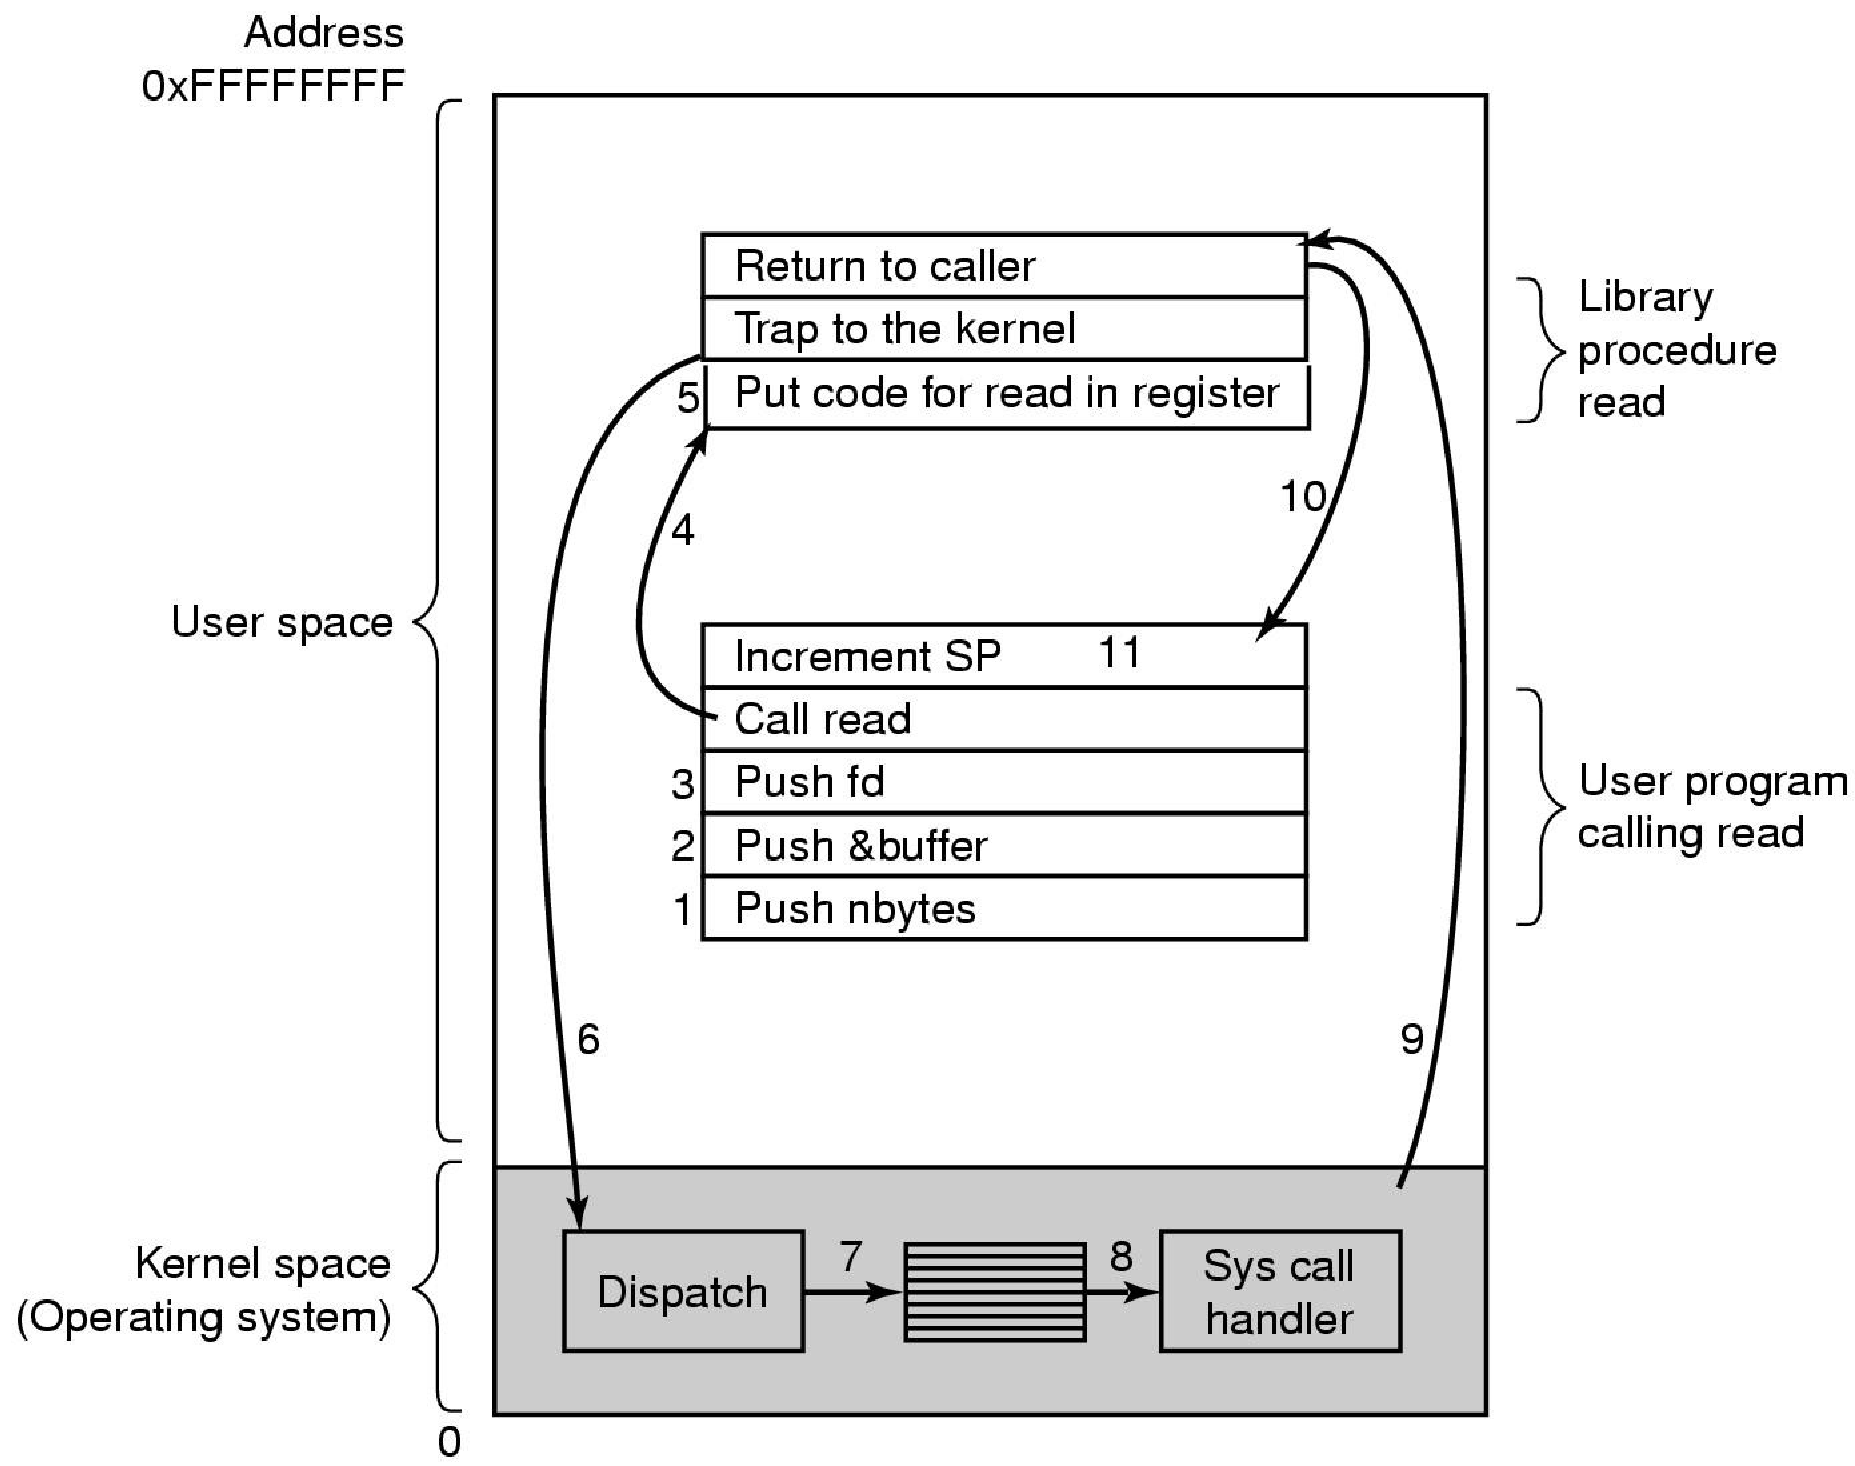
\includegraphics[width=0.7\textwidth]{library_call}
	\caption{Llamado a procedimientos de bibliotecas}
	\label{fig:library_call}
\end{figure}

Referencias de la Figura \ref{fig:library_call}:
\begin{itemize}
	\item 1, 2, 3 y 4 corresponden a un llamado convencional a un procedimiento.
	\item Antes de hacer 5, el sistema operativo habilita el acceso a la memoria del sistema operativo (pasa a modo kernel).
	\item 6 implica una software trap, el procesador pasa a modo protegido.
	\item 7 y 8 se ejecutan en modo protegido del procesador.
	\item En 9 se vuelve a modo usuario del procesador, pero con el sistema operativo en modo kernel.
	\item El paso 10 restablece la protección de memoria del sistema operativo (sale de modo kernel).
\end{itemize}

\newpage
\section{Procesos}
\subsection{Modelo de procesos}
El sistema operativo debe organizar el software que corre en unidades secuenciales, a esta organización se le llama proceso.\\

Un proceso es:
\begin{itemize}
	\item La imagen de un programa en ejecución (una copia del programa).
	\item Con las estructuras del sistema operativo para administrarlo.
	\item Varios procesos pueden estar asociados a un mismo programa; por ejemplo, iniciar varias instancias de un mismo programa generalmente significa que más de un proceso está siendo ejecutado.
\end{itemize}

Un proceso tiene:
\begin{itemize}
	\item La imagen del programa (una copia de su código ejecutable y de su área de datos).
	\item La información acerca de sus estado de ejecución:
	\begin{itemize}
		\item Los valores del program counter, registros y variables.
		\item Información necesaria para su administración por parte del Sistema Operativo (id, prioridad, ...).
	\end{itemize}
	\item Memoria (generalmente una región de memoria virtual); que incluye el código ejecutable, datos específicos del proceso (entrada y salida), un stack de llamadas (para mantener registro de las subrutinas activas y otros eventos), y un heap para mantener datos intermedios generados durante el tiempo de ejecución.
	\item Descriptores de recursos del sistema operativos, reservados por el proceso, como pueden ser los \emph{file descriptors} (Unix), o \emph{handles} (Windows), y fuentes y sumideros de datos.
	\item Atributos de seguridad, como el propietario del proceso y los permisos (operaciones permmitidas) del mismo.
\end{itemize}

Esta información la guarda el sistema operativo en estructuras de datos llamadas \emph{Process Control Blocks}.\\

Cualquier subgrupo de recursos, menos, generalmente, el estado del procesador, puede estar asociado con cada uno de los threads del proceso (en sistemas operativos que soportan threads) o en los procesos ``hijos''.

El sistema operativo mantiene sus procesos separados y reserva los recursos que necesitan, de manera que sean menos propensos a interferir entre ellos y causen fallas del sistema (como deadlocks o thrashing). El sistema operativo también provees mecanismos para la comunicación entre procesos, permitiéndoles interactuar de manera segura y predecible.

\subsection{Multiprogramación}
En computación, \emph{multitasking} es un método donde múltiples tareas (procesos) son ejecutadas durante el mismo periodo de tiempo. Se ejecutan \emph{concurrentes} (en periodos de tiempo solapados, una tarea puede iniciar antes que otras hayan terminado) en vez de \emph{secuenciales} (una tarea comienza luego de que la anterior haya terminado). Las tareas concurrentes comparten recursos de procesamiento, como la CPU y memoria principal.\\

Multitasking no necesariamente significa que varias tareas se ejecutan en el mismo preciso momento. En otras palabras, multitasking NO implica paralelismo, pero si significa que más de una tarea puede estar en medio de su ejecución al mismo tiempo, y que mas de una tarea está avanzando dentro de un período de tiempo determinado.

En caso de una computadora con un solo CPU, solo una tarea se dice estar corriendo en determinado tiempo, lo que significa que ese CPU está activamente ejecutando instrucciones para esa tarea.\\
Multitasking resuelve este problema organizando qué tarea se ejecutará en cada tiempo determinado, y cuándo una tarea en espera obtiene un turno. El acto de reasignar un CPU de una tarea a otra se llama \emph{context switch}, o cambio de contexto. Cuando estos cambios de contexto ocurren lo suficientemente seguidos, se logra una ilusión de paralelismo.

Incluso en computadoras con más de un CPU (máquinas \emph{multiprocesadores}) o más de un núcleo en determinado CPU (máquinas \emph{multinúcleo}), donde más de una tarea puede ser ejecutada en un determinado instante (una por núcleo), multitasking permite correr muchas más tareas que la cantidad de CPUs presentes.

Cuando hay más de un procesador se conoce como Multiprocesamiento.

Se ejecuta un proceso. Cuando se ``bloquea'' por I/O, se aprovecha el tiempo para ejecutar otro proceso.

La CPU va conmutando (switching) de un proceso a otro.

Es un multiplexado de la CPU.

\subsubsection{Implementación de la multiprogramación}
\begin{itemize}
	\item Se conoce como \emph{scheduler} al mecanismo que permite elegir varios procesos en estado \emph{Ready}, para otorgarles tiempo de CPU y que puedan realizar sus tareas. Para ello aplica un algoritmo de scheduling, que tiene en cuenta los siguientes aspectos
	\begin{itemize}
		\item Cantidad requerida de recursos.
		\item Cantidad actualmente disponible de recursos.
		\item Prioridad del trabajo o proceso.
		\item la cantidad de tiempo de espera.
	\end{itemize}
	
	\item \emph{Dispatcher} es el mecanismo que otorga tiempo de CPU al proceso seleccionado por el scheduler. Para esto, se realizan los siguientes pasos:
	\begin{itemize}
		\item Cambio de contexto (\emph{Context switching})
		\item Cambiar a modo usuario (\emph{user mode})
	\end{itemize}
	El tiempo se divide en segmentos, denominados \emph{time slices}. Cuando un \emph{time slice} se termina, le permite al scheduler actualizar el estado de cada proceso, y seleccionar el próximo a ejecutar.
\end{itemize}

Cada vez que se interrumpe un proceso también se pierde el tiempo de guardar el contexto.

\subsection{Estados de un proceso}
\begin{figure}[H]
	\centering
	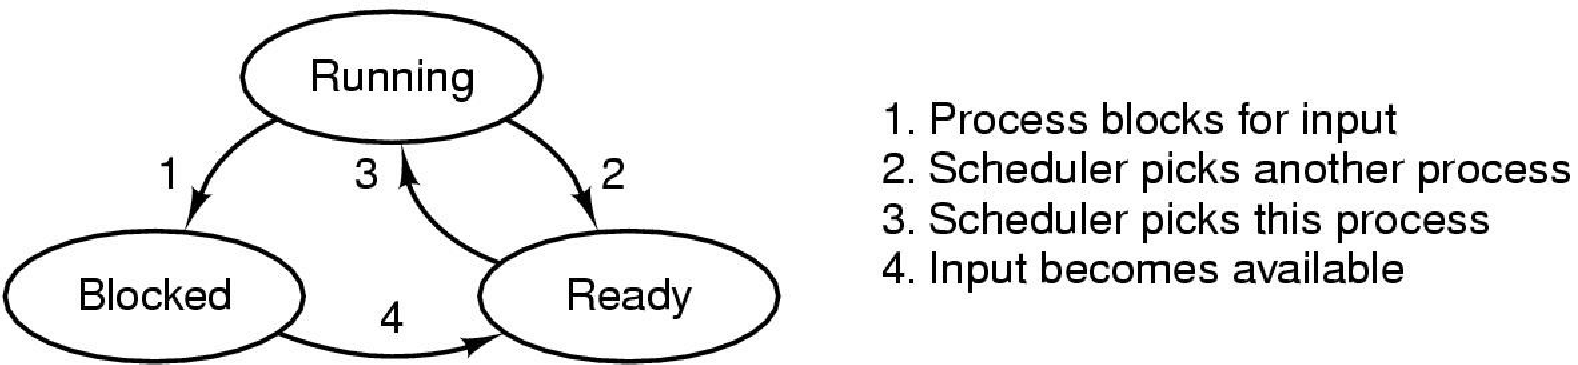
\includegraphics[width=0.7\textwidth]{process_states_simple}
	\caption{Estados de un procedimiento (simplificado)}
	\label{fig:process_states_simple}
\end{figure}

\begin{figure}[H]
	\centering
	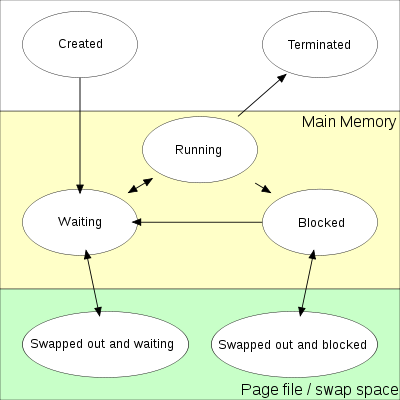
\includegraphics[width=0.5\textwidth]{process_states_full}
	\caption{Estados de un procedimiento}
	\label{fig:process_states_full}
\end{figure}

\subsubsection{Created or New}
When a process is first created, it occupies the ``created'' or ``new'' state. In this state, the process awaits admission to the ``ready'' state. This admission will be approved or delayed by a long-term, or admission, scheduler. Typically in most desktop computer systems, this admission will be approved automatically, however for real-time operating systems this admission may be delayed. In a real time system, admitting too many processes to the ``ready'' state may lead to oversaturation and over contention for the systems resources, leading to an inability to meet process deadlines.

\subsubsection{Ready and waiting}
A ``ready'' or ``waiting'' process has been loaded into main memory and is awaiting execution on a CPU (to be context switched onto the CPU by the dispatcher, or short-term scheduler). There may be many ``ready'' processes at any one point of the system's execution—for example, in a one-processor system, only one process can be executing at any one time, and all other ``concurrently executing'' processes will be waiting for execution.

A ready queue or run queue is used in computer scheduling. Modern computers are capable of running many different programs or processes at the same time. However, the CPU is only capable of handling one process at a time. Processes that are ready for the CPU are kept in a queue for ``ready'' processes. Other processes that are waiting for an event to occur, such as loading information from a hard drive or waiting on an internet connection, are not in the ready queue.

\subsubsection{Running}
A process moves into the running state when it is chosen for execution. The process's instructions are executed by one of the CPUs (or cores) of the system. There is at most one running process per CPU or core. A process can run in either of the two modes, namely kernel mode or user mode.

\subsubsection{Blocked (Waiting)}
A process that is blocked on some event (such as I/O operation completion or a signal). A process may be blocked due to various reasons such as when a particular process has exhausted the CPU time allocated to it or it is waiting for an event to occur.

\subsubsection{Terminated}
A process may be terminated, either from the ``running'' state by completing its execution or by explicitly being killed. In either of these cases, the process moves to the ``terminated'' state. The underlying program is no longer executing, but the process remains in the process table as a zombie process until its parent process calls the wait system call to read its exit status, at which point the process is removed from the process table, finally ending the process's lifetime. If the parent fails to call wait, this continues to consume the process table entry (concretely the process identifier or PID), and causes a resource leak.\\

A child process always first becomes a zombie before being removed from the resource table. In most cases, under normal system operation zombies are immediately waited on by their parent and then reaped by the system – processes that stay zombies for a long time are generally an error and cause a resource leak.\\

Después de terminado un proceso, el mismo queda en estado ``terminado'' hasta que el sistema operativo termina de limpiar las estructuras que usó para ejecutarlo (mientras tanto está en estado zombie).

\begin{lstlisting}
int main()
{
	pid_t child_pid;

	child_pid = fork();
	if(child_pid > 0){
		sleep(60);
	}else{
		exit(0);
	}
	return 0;
}
\end{lstlisting}

\subsection{PCB (Process Control Block)}
Es la estructura de datos con la que el sistema operativo administra los procesos.
Contiene la información acerca del proceso y su estado.
Además la información que el SO precisa para manejarlo como: Identificador, Estado, Recursos, Historia.
Ejemplo de datos que maneja: Registros, Program counter, Process ID, Punteros de memoria, etc.

\underline{Estados de un proceso}:
Los estados se manejan como colas.
El Dispatcher es el encargado de cambiar los PCBs entre las colas.

\subsubsection{Dispatcher (Scheduler de corto plazo)}
Decide qué proceso, entre los procesos en memoria y con estado \emph{ready}, será ejecutado (otorgado un CPU) luego de una interrupción del clock, una interrupción de entrada/salida, llamada al sistema operativo u otro tipo de señal. Por este motivo, este scheduler de corto plazo realizar tareas de planificación mucho más seguido que los schedulers de medio y largo plazo. Al menos una decisión de scheduling se realiza luego de cada \emph{time slice}, y estos son bastante cortos.

\begin{itemize}
	\item Al pasar de Running a Blocked.
	El manejador de interrupciones lo invoca para cambiar de estado al proceso:
	\begin{itemize}
		\item Salva los datos necesarios en el PCB.
		\item Cambia el PCB de cola.
	\end{itemize}
	Luego se decide a que proceso dar control (tarea del Scheduler).

	\item Al pasar de Ready a Running \\
	El Scheduler lo invoca cuando ya decidió a que proceso activar. \\
	Carga el estado de la CPU con los datos del PCB. \\
	Continúa la ejecución del proceso.
\end{itemize}

\subsubsection{Scheduler (Long term)}
Decide a cuál de los procesos en ready hay que darle el control.
In general, most processes can be described as either I/O-bound or CPU-bound. An I/O-bound process is one that spends more of its time doing I/O than it spends doing computations. A CPU-bound process, in contrast, generates I/O requests infrequently, using more of its time doing computations.
It is important that a long-term scheduler selects a good process mix of I/O-bound and CPU-bound processes. If all processes are I/O-bound, the ready queue will almost always be empty, and the short-term scheduler will have little to do. On the other hand, if all processes are CPU-bound, the I/O waiting queue will almost always be empty, devices will go unused, and again the system will be unbalanced.
he system with the best performance will thus have a combination of CPU-bound and I/O-bound processes.\\

Tiene en cuenta las características del proceso:

\begin{itemize}
	\item \textbf{Throughput} - The total number of processes that complete their execution per time unit.
	\item \textbf{Latency}, specifically:
	\begin{itemize}
		\item \textbf{Turnaround time} - total time between submission of a process and its completion.
		\item \textbf{Response time} - amount of time it takes from when a request was submitted until the first response is produced.
	\end{itemize}
	\item \textbf{Fairness} - Equal CPU time to each process (or more generally appropriate times according to each process' priority and workload).
	\item \textbf{Waiting Time} - The time the process remains in the ready queue.
\end{itemize}

\paragraph{Objetivos del Scheduler:}
\begin{itemize}
	\item Dar una participación adecuada del reparto de tiempo de CPU (Fairness).
	\item Equilibrar el uso de recursos (Load Balancing).
	\item Aplicar las políticas generales del Sistema (prioridades, afinidad, seguridad).
	\item El resto depende del tipo de Sistema.
\end{itemize}

In practice, these goals often conflict (e.g. throughput versus latency), thus a scheduler will implement a suitable compromise. Preference is given to any one of the concerns mentioned above, depending upon the user's needs and objectives.

\begin{itemize}
	\item Batch (por lotes):
	\begin{itemize}
		\item maximizar el throughput: cantidad de procesos / tiempo.
		\item Mantener la CPU ocupada.
		\item Minimizar el turnaround time.
	\end{itemize}
	\item Interactivo:
	\begin{itemize}
		\item Buen tiempo de respuesta
		\item Expectativas del usuario
	\end{itemize}
	\item Real time:
	\begin{itemize}
		\item Cumplir con los deadlines
		\item Desempeño predecible
	\end{itemize}
\end{itemize}

Las decisiones de scheduling se pueden tomar cuando un proceso:

\begin{itemize}
	\item Pasa de running a blocked/waiting. (Transicion NO apropiativa)
	\item Pasa de running a ready. (Transicion apropiativa)
	\item Pasa de blocked/waiting a ready. (apropiativa)
	\item Termina. (NO apropiativa)
\end{itemize}

\textbf{Transición apropiativa}: es el SO el que interrumpe.

\textbf{Transición no apropiativa}: es el propio proceso el que interrumpe.

\textbf{Starvation}: es un problema que ocurre cuando hay multitasking, donde a un proceso se le niega constantemente los recursos necesarios. De esta manera la tarea nunca puede concretarse.

\subsection{Algoritmos de scheduling}

\begin{enumerate}
	\item FIFO
	\item Shortest Job Next (SJN)
	\item Round Robin
	\item Múltiples colas con prioridad
\end{enumerate}

\subsubsection{First come-First served (FIFO)}
Simplemente encola procesos en estado \emph{ready} en el orden de llegada.\\

\textbf{Características}

\begin{itemize}
	\item Since context switches only occur upon process termination, and no reorganization of the process queue is required, scheduling overhead is minimal.
	\item Throughput can be low, since long processes can hold the CPU
	\item Turnaround time, waiting time and response time can be high for the same reasons above
	\item No prioritization occurs, thus this system has trouble meeting process deadlines.
	\item The lack of prioritization means that as long as every process eventually completes, there is no starvation. In an environment where some processes might not complete, there can be starvation.
	\item It is based on Queuing
\end{itemize}

\subsubsection{Shortest Job Next}
Selecciona para ser ejecutado el proceso en espera con el menor tiempo de ejecución.

\textbf{Pros}:
\begin{itemize}
	\item Shortest job next is advantageous because of its simplicity and because it minimizes the average amount of time each process has to wait until its execution is complete. 
\end{itemize}

\textbf{Contras}:
\begin{itemize}
	\item However, it has the potential for process starvation for processes which will require a long time to complete if short processes are continually added.
	\item Another disadvantage of using shortest job next is that the total execution time of a job must be known before execution. While it is not possible to perfectly predict execution time, several methods can be used to estimate the execution time for a job, such as a weighted average of previous execution times.
\end{itemize}

\subsubsection{Round Robin}
Time slices are assigned to each process in equal portions and in circular order, handling all processes without priority (also known as cyclic executive). 

\textbf{Pros}:
\begin{itemize}
	\item Round-robin scheduling is simple, easy to implement, and starvation-free.
	\item Good average response time, waiting time is dependent on number of processes, and not average process length.
	\item Starvation can never occur, since no priority is given. Order of time unit allocation is based upon process arrival time, similar to FCFS.
\end{itemize}

\textbf{Contras}:
\begin{itemize}
	\item Because of high waiting times, deadlines are rarely met in a pure RR system.
\end{itemize}

\subsubsection{Múltiples colas con Prioridad}
This is used for situations in which processes are easily divided into different groups. For example, a common division is made between foreground (interactive) processes and background (batch) processes. These two types of processes have different response-time requirements and so may have different scheduling needs. It is very useful for shared memory problems.
If a process uses too much CPU time, it will be moved to a lower-priority queue. This scheme leaves I/O-bound and interactive processes in the higher priority queues. In addition, a process that waits too long in a lower-priority queue may be moved to a higher priority queue. This form of aging also helps to prevent starvation of certain lower priority processes.

\subsection{Creacion/Terminacion de procesos}
\subsubsection{Creación de Procesos}
\begin{itemize}
	\item Al iniciar el sistema (Booting)
	\item Por pedido del usuario (Uso de una System Call).
\end{itemize}

\subsubsection{Terminación de procesos}
\begin{itemize}
	\item Salida normal (voluntaria).
	\item Salida por error (voluntaria).
	\item Error ``fatal'' (involuntaria).
	\item ``Muerte'' por otro proceso.
\end{itemize}

\subsection{Booting}
A boot loader is a computer program that loads an operating system or some other system software for the computer after completion of the power-on self-tests; it is the loader for the operating system itself, which has its own loader for loading ordinary user programs and libraries. Within the hard reboot process, it runs after completion of the self-tests, then loads and runs the software. A boot loader is loaded into main memory from persistent memory, such as a hard disk drive or, in some older computers, from a medium such as punched cards, punched tape, or magnetic tape. The boot loader then loads and executes the processes that finalize the boot.

\begin{itemize}
	\item Cargar en memoria un software que pueda lanzar un Sistema Operativo.
	\begin{itemize}
		\item Switches en el panel.
		\item Flash boot loader.
		\item MBR (Master Boot Record) program.
		\item EFI (Extended Firmware Interface).
	\end{itemize}
	\item Termina cargando el first stage boot loader.
\end{itemize}

\subsection{EFI (Extensible Firmware Interface)}
Interfaz Extensible del Firmware, Extensible Firmware Interface (EFI), es una especificación desarrollada por Intel dirigida a reemplazar la antigua interfaz del estándar IBM PC ROM BIOS, e interactúa como puente entre el sistema operativo y el firmware base.

\begin{itemize}
	\item Boot Services:
	\begin{itemize}
		\item Soporte de consola.
		\item Soporte gráfico.
	\end{itemize}
	\item Runtime Services:
	\begin{itemize}
		\item Device Drivers
		\item Fecha y Hora
	\end{itemize}
	\item Carga de código desde Internet
\end{itemize}

Las especificaciones de la EFI permiten ofrecer un controlador de dispositivo independiente del procesador denominado EFI Byte Code o simplemente EBC. Gracias a esto, se permite soporte para la carga de gráficos, red, sonido y opciones avanzadas del sistema, sin haber precargado el sistema operativo en cuestión. Esto era totalmente imposible en el BIOS, ya que cargaba funciones muy limitadas y necesarias como el soporte de periféricos como teclado y ratón.

\subsection{UEFI}
El 25 de julio de 2005 se creó la fundación UEFI (Unified Extensible Firmware Interface) cuya labor consistía en desarrollar y promocionar la plataforma EFI.

Define un “boot manager” (a firmware policy engine) que carga el loader del SO y los drivers que se necesiten.
La configuración del booteo se almacena en variables NVRAM (path de loaders)
Los loaders del SO son “clases” de aplicaciones UEFI, como clases que son, se almacenan en el file system (EFI System partition) que es independiente del medio (HD, Optical Disk, etc).
Especifica un Shell para ejecutar aplicaciones (eje boot loaders), modificar variables, etc
Mantiene compatibilidad reversa con BIOS

\subsection{Proceso de BOOT – Linux}
En Linux, el flujo de control durante el arranque es desde el BIOS, al gestor de arranque y al núcleo (kernel). 
El núcleo inicia el planificador (para permitir la multitarea) y ejecuta el primer espacio de usuario (es decir, fuera del espacio del núcleo) y el programa de inicialización (que establece el entorno de usuario y permite la interacción del usuario y el inicio de sesión), momento en el que el núcleo se inactiva hasta que sea llamado externamente.

\subsection{Creación de procesos por el usuario}
Espacio de direcciones de un proceso

\begin{itemize}
	\item TXT: Ejecutable
	\item DATA: Variables ``static''
	\item U\_Area: Stack + Información del proceso
\end{itemize}

\subsubsection{TXT}
The Text segment (a.k.a the Instruction segment) contains the executable program code and constant data. The text segment is marked by the operating system as read-only and can not be modified by the process. Multiple processes can share the same text segment. Processes share the text segment if a second copy of the program is to be executed concurrently.

\subsubsection{Data}
The data segment, which is contiguous (in a virtual sense) with the text segment, can be subdivided into initialized data (e.g. in C/C++, variables that are declared as static or are static by virtual of their placement) and uninitialized (or 0-initizliazed) data. The uninitialized data area is also called BSS (Block Started By Symbol). For example, Initialized Data section is for initialized global variables or static variables, and BSS is for uninitialized.

\subsubsection{U\_Area (STACK + Process info)}
In addition to the text, data, and stack segment, the OS also maintains for each process a region called the u area (User Area). The u area contains information specific to the process (e.g. open files, current directory, signal action, accounting information) and a system stack segment for process use. If the process makes a system call (e.g., the system call to write in the function in main ), the stack frame information for the system is stored in the system stack segment. Again, this information is kept by the OS in an area that the process doesn't normally have access to. Thus, if this information is needed, the process must use special system call to access it. Like the process itself, the contents of the u area for the process are paged in and out by the OS.

\subsection{Fork y Exec}
\subsubsection{Exec}
Reemplaza al proceso actual con un nuevo programa.

\subsubsection{Fork}
Lanza un nuevo proceso a imagen y semejanza de sí mismo. El hijo tiene el mismo código ejecutable que su padre.
The fork operation creates a separate address space for the child
When a process calls fork, it is deemed the parent process, and the newly created process, its child. After the fork, both processes not only run the same program, but they resume execution as though both had called the system call. They can then inspect the call's return value to determine their status, child or parent, and act accordingly.
Cada uno tiene su propio espacio de direcciones. No se comparte memoria de escritura.

So, \texttt{fork()} and \texttt{exec()} are often used in sequence to get a new program running as a child of a current process. Shells typically do this whenever you try to run a program like \texttt{find} - the shell forks, then the child loads the \texttt{find} program into memory, setting up all command line arguments, standard I/O and so forth.\\

\textbf{Laboratorio}

\begin{lstlisting}
if ( (pidhijo = fork()) == 0) {
	// When fork() returns 0, we are in the child process.
	cout << endl << "---> Es el HIJO con pid = " << getpid() << " cuyo padre es pid = " << getppid() << endl;
	exit(0);
} else {
	// When fork() returns a positive number, we are in the parent process
	// and the return value is the PID of the newly created child process.
	cout << endl << "Es el PADRE con pid = " << getpid() << " y su hijo es pid = " << pidhijo << endl;
	exit(0);
}
\end{lstlisting}

Fork copia TXT, Data y U\_Area “on demand”

\begin{lstlisting}
if (fork()==0){
	Read	//lee el hijo
} else {
	Read	//lee el padre
}
\end{lstlisting}

Los dos leen del mismo archivo. Si leen una vez cada uno, cada uno lee salteado.

\textbf{Lock compartido}: Asociado al read.
\textbf{Lock exclusivo}: Asociado al write.

Si quiero bloquear un archivo (de forma exclusiva) y ya esta bloqueado, se queda esperando hasta que se desbloquea.

El único caso en que los bloquea al mismo tiempo es que ambos sean compartidos.

El bloqueo no es una cola. Lo hace o se queda esperando, sin orden de prioridad.

El lock es un protocolo o una convención, pero no impide read, write, delete, etc, si se lo hace sin locks.\\

\textbf{Ejecución Foreground con proceso hijo Unix}
\begin{lstlisting}[language=sh]
> script1.sh 	#script1.sh necesita permiso de ejecución
# no nos devuelve el control hasta que no finaliza
\end{lstlisting}

\textbf{Ejecución Background con proceso hijo}
\begin{lstlisting}[language=sh]
> script1.sh & 		#script1.sh necesita permiso de ejecución
#Nos devuelve el control en el momento

[1] 20295 		#muestra el número de proceso
[1] + Done script1.sh 	#nos avisa que finalizó
\end{lstlisting}

\textbf{Ejecución Foreground sin proceso hijo}
\begin{lstlisting}[language=sh]
> . .script1.sh 		#script1.sh no necesita permiso de ejecución
#no nos devuelve el control hasta que no finaliza
#se ejecuta en el mismo ambiente, eso significa que
#no hay un shell hijo
\end{lstlisting}

\newpage
\section{Threads}
Los thread son mini-procesos en el mismo espacio de direcciones que corren casi en paralelo. Como están en el mismo espacio de direcciones, comparten la data. Es decir, son hilos de ejecución que comparten el agrupamiento de recursos.

Son más livianos que los procesos, así es que es más fácil y rápido crearlos y destruirlos.\\

Threads differ from traditional multitasking operating system processes in that:
\begin{itemize}
	\item processes are typically independent, while threads exist as subsets of a process
	\item processes carry considerably more state information than threads, whereas multiple threads within a process share process state as well as memory and other resources
	\item processes have separate address spaces, whereas threads share their address space
	\item processes interact only through system-provided inter-process communication mechanisms
	\item context switching between threads in the same process is typically faster than context switching between processes.
\end{itemize}

Cada thread tiene sus propios program counters, registros donde almacena sus variables,su stack y su estado. Pero comparten code, data y files.\\

Different threads in a process are not as independent as different processes. All threads have exactly the same address space, which means that they also share the same global variables. Since every thread can access every memory address within the process’ address space, one thread can read, write, or even wipe out anothre thread’s stack. There is no protection between threads because should not be necessary. All threads are owned by a single user, who has presumably created multiple threads so that the can cooperate, not fight. In addition to sharing an address space, all the threads can share the same set of open files, child processes, alarms, and signals.

\begin{figure}[H]
	\centering
	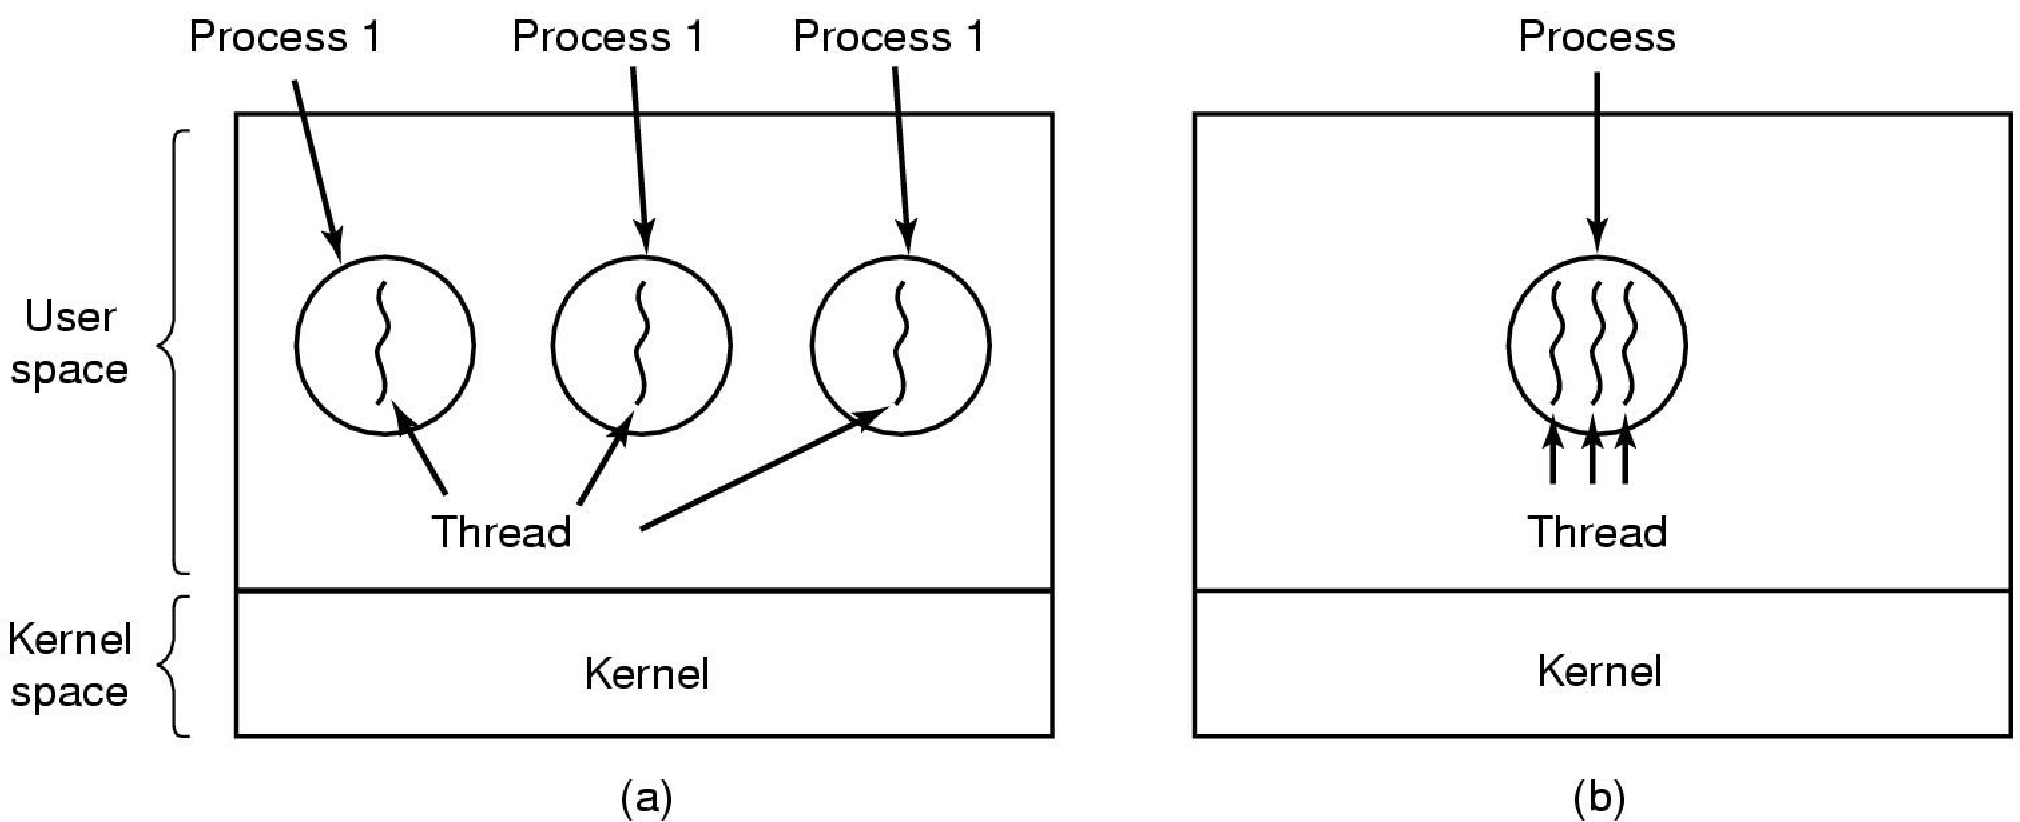
\includegraphics[width=0.66\textwidth]{differences_between_processes_and_threads_1}
	%\caption{Diferencia entre procesos y threads}
	\label{fig:differences_between_processes_and_threads_1}
\end{figure}

\begin{figure}[H]
	\centering
	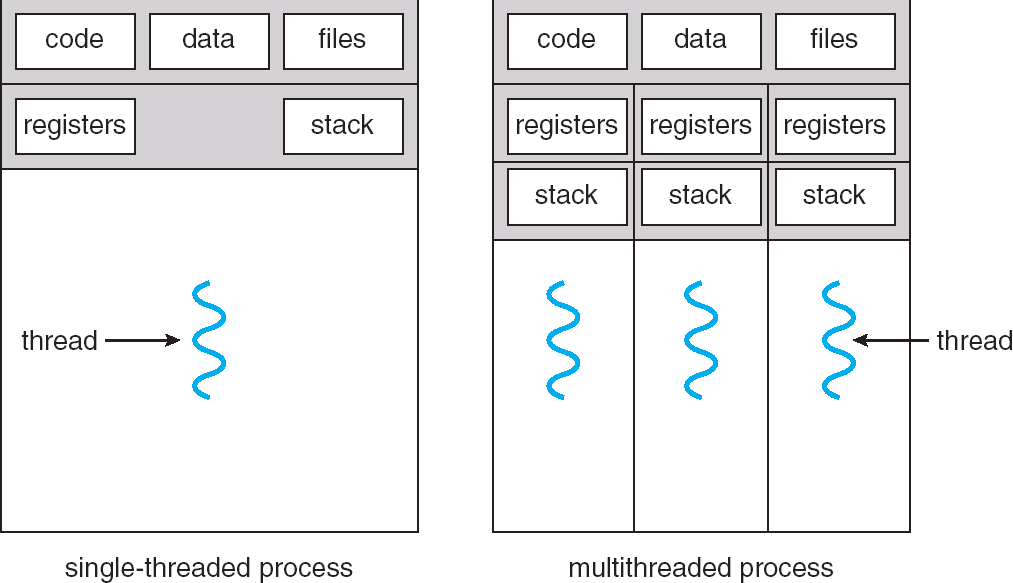
\includegraphics[width=0.65\textwidth]{differences_between_processes_and_threads_2}
	%\caption{Diferencia entre procesos y threads}
	\label{fig:differences_between_processes_and_threads_2}
\end{figure}

\textbf{Thread Control Block (TCB)}

Hay información que pasa del PCB al (o los) TCB

\begin{figure}[H]
	\centering
	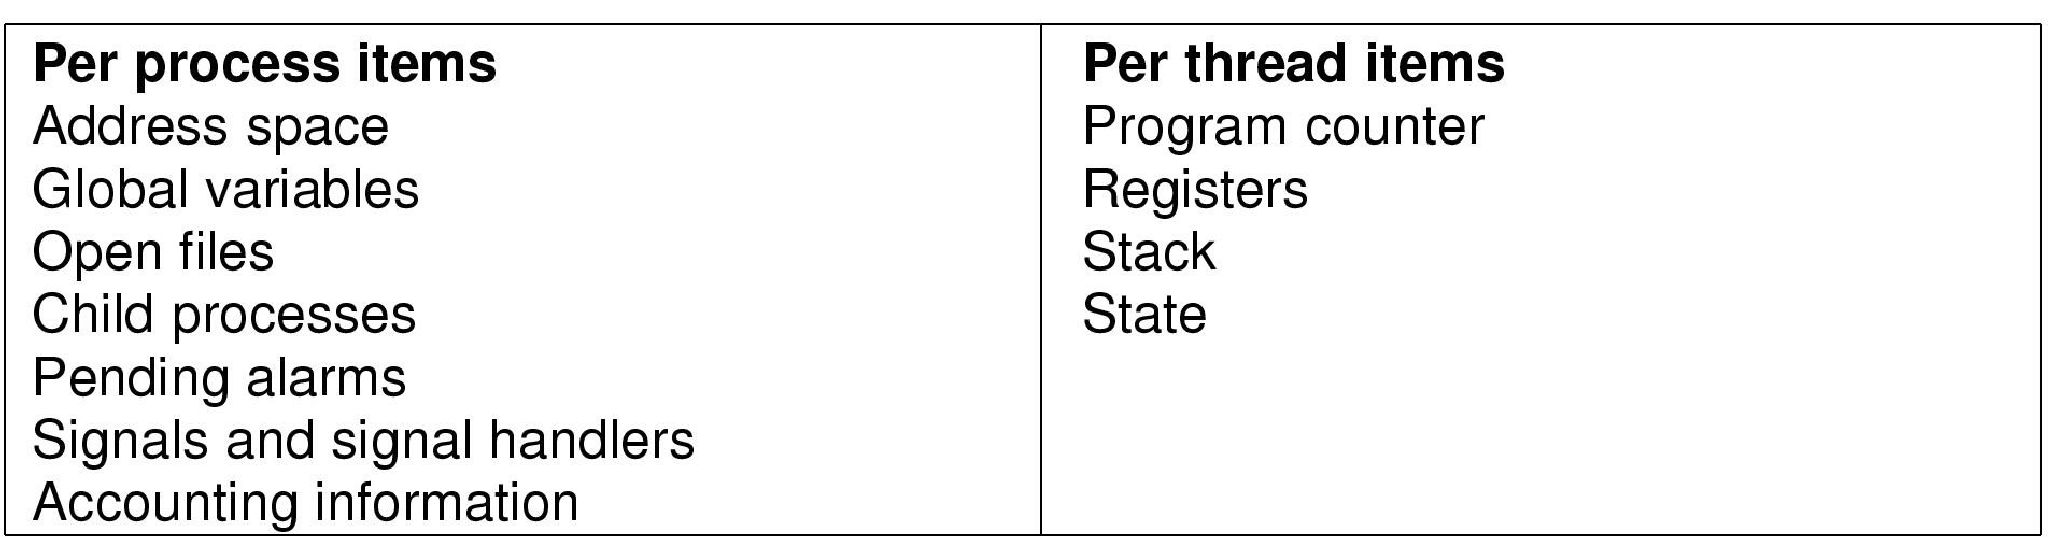
\includegraphics[width=0.7\textwidth]{differences_between_processes_and_threads_3}
	%\caption{Diferencia entre procesos y threads}
	\label{fig:differences_between_processes_and_threads_3}
\end{figure}

Like traditional process, thread can be in any of several states: running, blocked, ready or terminated. A running thread concurrently has the CPU and is active. A blocked thread is waiting for some event (or other thread) to unblock it. A ready thread is scheduled to run and will as soon as its turn come up. The transitions between threads states are the same as transitions between process states.

\subsection{Aplicaciones de multithreading}
Varias aplicaciones que concurren sobre los mismo datos como:
\begin{itemize}
	\item Un server que lanza un thread por cada pedido.
	\item Un procesador de texto concurrente con su corrector y su armador de pagina.
	\item El manejo de Interfaces Gráficas.
\end{itemize}

Algunos de los sistemas hechos con threads podrían hacerse con eventos.

Eventos usan handlers y callbacks, los threads quedan congelados hasta que se les devuelve el control.

Escalar con threads es casi trivial, escalar con eventos tiene un techo (stack ripping).

No mezclar threads con eventos.

\subsection{Implementacion de threading}
There are two main ways to implement a threads package: in user space and in the kernel (a hybrid implementation is also possible).

\subsubsection{Threads in user space}
The kernel knows nothing about them. As far as the kernel is concerned, it is managing ordinary, single-threaded processes (can be implemented in operating systems than not suport threading). Threads are implemented by a library.

Cada proceso tiene su propia tabla de threads privada, para seguir el rastro a cada uno de sus threads. En la tabla se guardan las propiedades del thread (program counter, stack pointer, registers, state, etc). La tabla es manejada por el runtime system.

When a thread does something that may cause it to become blocked locally, for example, waiting for another thread in its process to complete some work, it calls a run-time system procedure. This procedure checks to see if the thread must be put in a blocked state. If so, it stores the thread’s registers in the thread table, looks in the table for a ready thread to run, and reloads the machine registers with the new thread’s saved values. As soon as the stack pointer and program counter have been switched, the new thread comes to life again automatically.

La biblioteca de threads permite al usuario multiplexar su time slice.

Time slice: tiempo que puede ejecutarse un proceso sin que el SO lo pare (impide que el usuario bloquee el sistema).\\

\textbf{Ventajas}
\begin{itemize}
	\item Doing thread switching like this is at least an order of magnitude (maybe more) faster than trapping to the kernel. The procedure that saves the thread’s state and the scheduler are just local procedures, so invoking them is much more efficient than making a kernel call. Among other issues, no trap is needed, no context switch is needed, the memory cache need not be flushed, and so on. This makes thread scheduling very fast.
	\item Customized scheduling algorithm.
	\item Scale better, since kernel threads require some table space and stack space in the kernel, which can be a problem if there are a very large number of threads.
\end{itemize}

\textbf{Problemas}
\begin{itemize}
	\item How to implement blocking systems calls. It should prevent one blocked thread from affecting others.
	\item If a thread starts running, no other thread in that process will ever run unless the first thread voluntarily gives up the CPU
\end{itemize}

\begin{figure}[H]
	\centering
	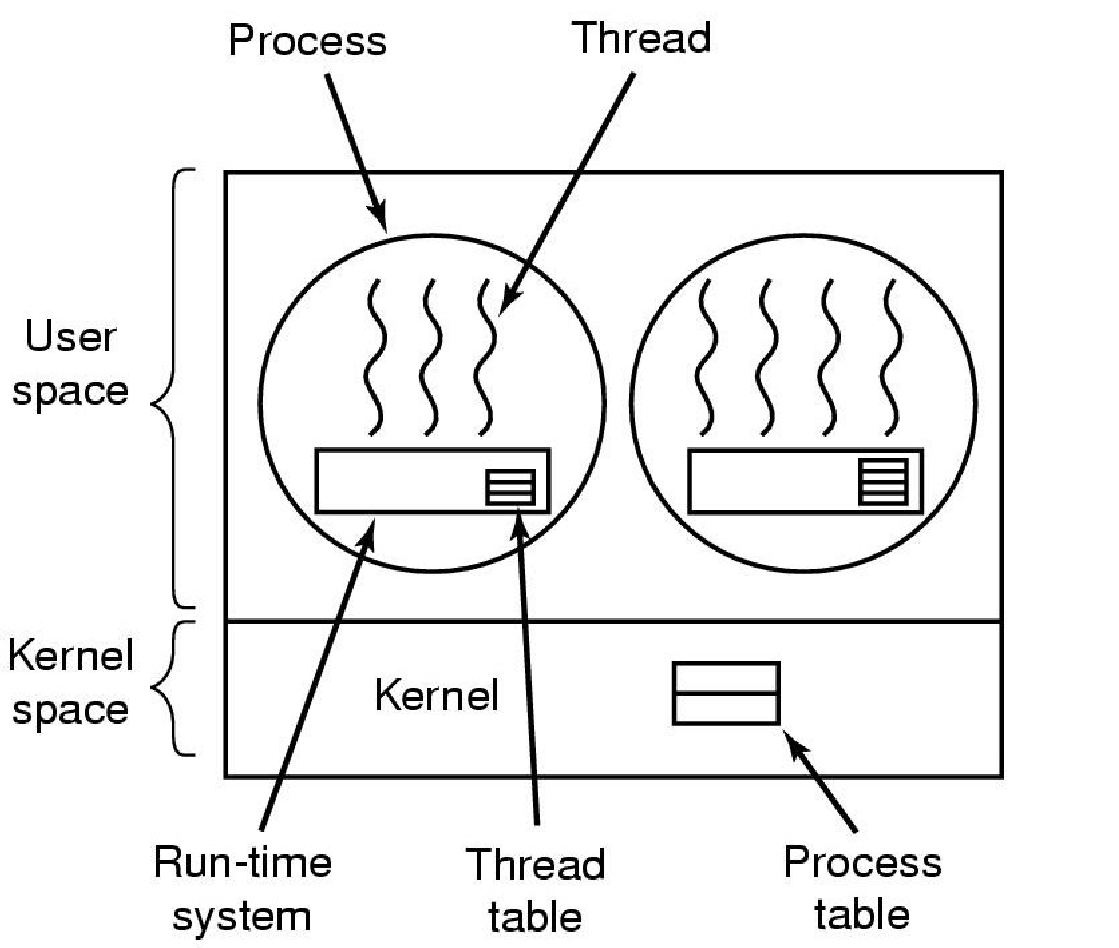
\includegraphics[width=0.5\textwidth]{threads_user_space}
	\caption{Threads en el espacio de usuario}
	\label{fig:threads_user_space}
\end{figure}

\subsubsection{Kernel threads}
The kernel has a thread table that keeps track of all the threads in the system. When a thread wants to create a new thread or destroy an exisiting one, it makes a kernel call, which then does the creation or destruction by updating the kernel thread table.

La tabla del kernel es igual a la que se usa en los threads en el espacio de usuario, pero almacenada en el kernel.

All calls that might block a thread are implemented as system calls, at considerably greater cost than a call to a run-time system procedure. When a thread blocks, the kernel, at its options, can run either another thread from the same process (if one is ready) or a thread from a different process. With user-level threads, the run-time system keeps running threads from its own process until the kernel takes the CPU away from it (or there are no ready threads left to run).

Due to the relatively greater cost of creating and destroying threads in the kernel, some systems recycle their threads. When a thread is destroyed, it is marked as not runnable, but its kernel data structures are not otherwise affected. Later, when a new thread must be ccreated, and old thread is reactivated, saving some overhead.

Kernel threads do not require any new, nonblocking system calls.

Their main disadvantage is that the cost of a system call is substantial, so if thread operations (creation, termination, etc) are common, much more overhead will be incurred.\\

\textbf{Some problems}
\begin{itemize}
	\item Multithreaded process fork: How many threads for the new one?
	\item Signals: when a signal comes in, which thread should handle it?
\end{itemize}

\begin{figure}[H]
	\centering
	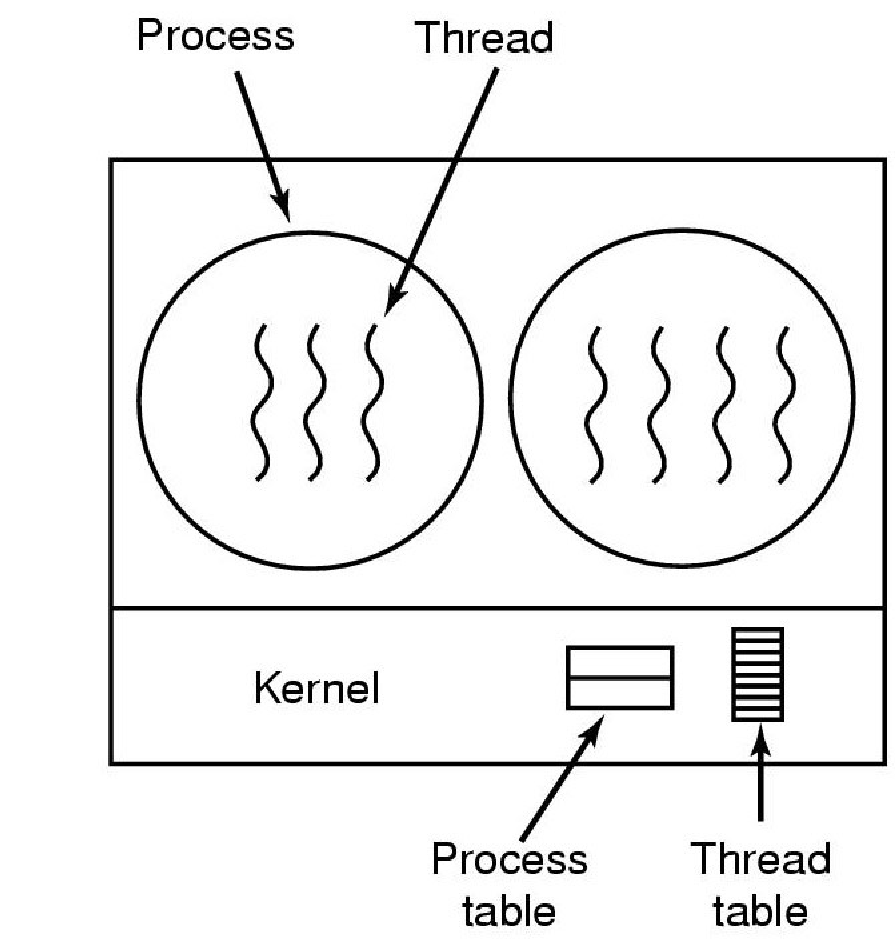
\includegraphics[width=0.5\textwidth]{kernel_threads}
	\caption{Kernel Threads}
	\label{fig:kernel_threads}
\end{figure}

\subsubsection{Implementaciones hibridas}
One way is use kernel-level threads and then multiplex user-level threads onto some or all the kernel threads. The programmer can determine how many kernel threads to use and how many user-level threads to multiplex on each one.

The kernel is aware of only the kernel-level threads and schedules those. Some of those threads may have multiple user-level threads multiplexed on top of them. These user level threads are created, destroyed and scheduled just like user-level threads in a process.Each kernel-level thread has some set of user-level threads that take turns using it.

\begin{figure}[H]
	\centering
	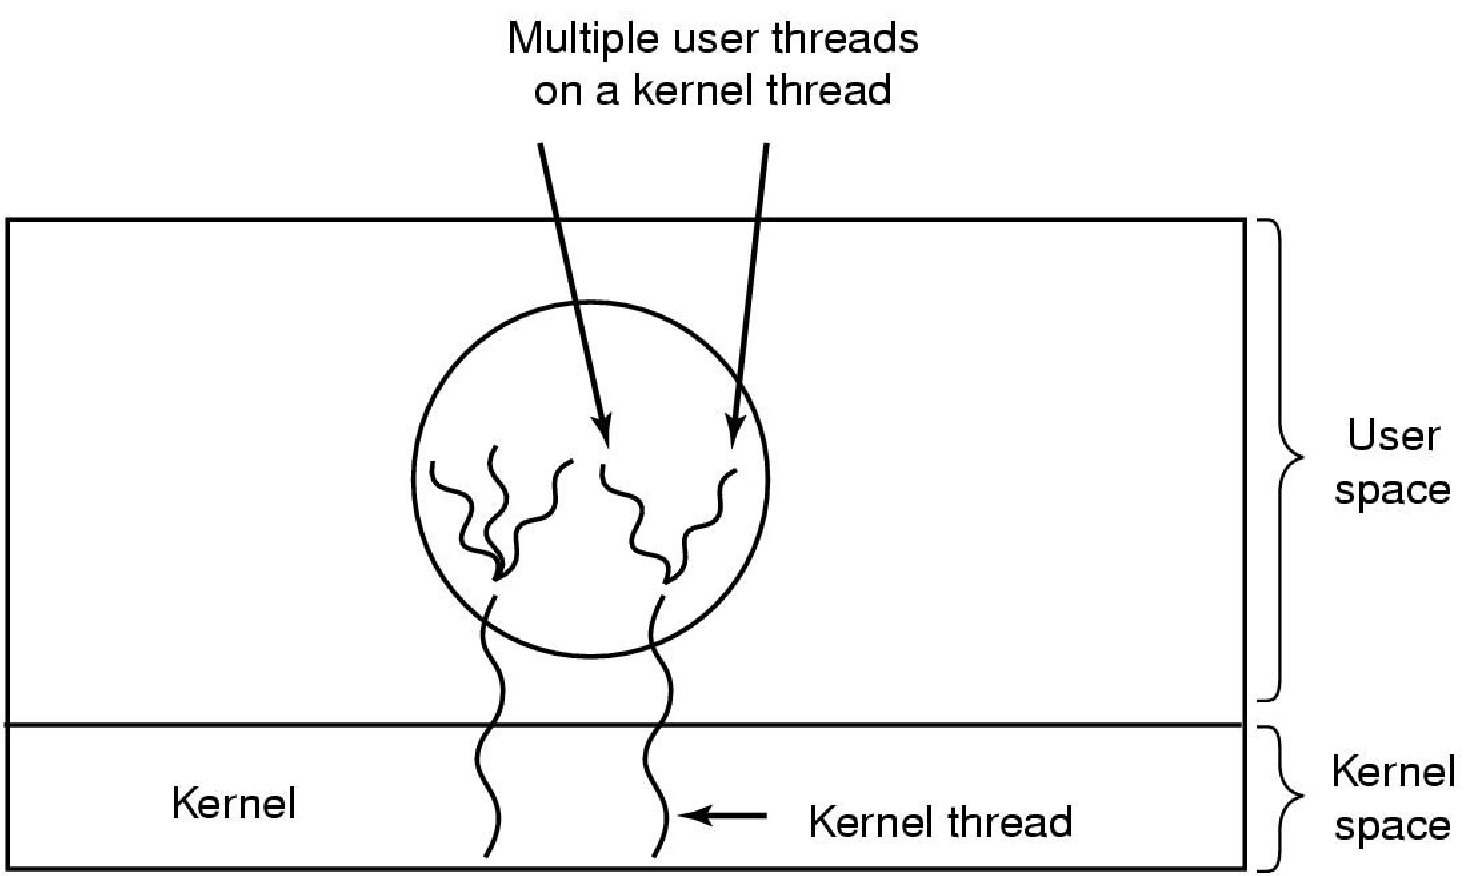
\includegraphics[width=0.5\textwidth]{hybrid_threads}
	\caption{Threads híbridos}
	\label{fig:hybrid_threads}
\end{figure}

\textbf{Scheduler activations}

Mimic the funcionality of kernel threads but with better performance (similar to user space threads).
Cuando se produce una interrupcion, el SO le devuelve el control al usuario.

The kernel assigns a certain number of virtual processors to each process and lets the user space runtime system allocate threads to processors.

The basic idea is that when the kernel knows that a thread has blocked, the kernel notifies the process runtime system by an “upcall”. The runtime system, at its own discretion, can either restart the blocked thread immediately or put it on the ready list to be run later.

An objection to scheduler activations is the fundamental reliance on upcalls, a concept tha violates the structure inherent in any layered system. Normally, layer n offers certain services that layer n+1 can call on, but layer n may not call procedures in layer n + 1. Upcalls do not follow this fundamental principle.

\newpage
\section{Administracion de memoria}
\subsection{Definición}
Suministrar la memoria necesaria para el código de un programa y sus estructuras de datos. Esto incluye:
\begin{itemize}
	\item Asignación de memoria.
	\item Reciclado del almacenamiento.
\end{itemize}

Está relacionado con el esquema de manejo de memoria soportado por el lenguaje, el compilador se encarga de intercalar el código correspondiente.

\subsection{Vocabulario de manejo de memoria en los lenguajes}
\begin{description}
	\item[Declarar una variable] Establecer nomenclatura (introducir el identificador) sin asignar memoria. Es un paso necesario pero no suficiente para usarla.
	
	\item[Definir una variable] Asignarle memoria y posiblemente un valor inicial. Se puede usar una vez que está definida.
	
	\item[Ambiente] Porción de código durante el cual una variable está declarada.
	
	\item[Vida] Intervalo de la ejecución en el cual una variable tiene memoria asignada.
	
	\item[Ámbito (scope)] Cuando una variable está en su ambiente y en su tiempo de vida. Es en tiempo de ejecución.
\end{description}

\subsection{Tipos de variables según su manejo en memoria}
\subsubsection{Externa}
Se encuentra definida pero no declarada en el bloque.
Debido a que las variables externas son accesibles globalmente, puede ser utilizadas para comunicar datos entre funciones, en lugar de una lista de parámetros.
Además, como las variables externas permanecen en existencia, en vez de aparecer y desaparecer a lo largo de las llamadas y salidas de las funciones, retienen sus valores incluso después que las funciones que las funciones que le asignaron valor salieron.

\subsubsection{Estática}
Su vida se extiende a toda la duración del programa.
When a program (executable or library) is loaded into memory, static variables are stored in the data segment of the program's address space (if initialized), or the BSS segment (if uninitialized), and are stored in corresponding sections of object files prior to loading.
In terms of scope and extent, static variables have extent the entire run of the program, but may have more limited scope. A basic distinction is between a static global variable, which has global scope and thus is in context throughout the program, and a static local variable, which has local scope and thus is only in context within a function (or other local context).

\subsubsection{Dinámica Automática}
La memoria se asigna y libera automáticamente cuando la ejecución ingresa en el ámbito de la variable.
Is a variable which is allocated and deallocated automatically when program flow enters and leaves the variable's context. No lo hace el programador, sino el compilador del lenguaje o una biblioteca.

\subsubsection{Dinámica Controlada}
La ejecución del programa (el programador) controla explícitamente cuando se asigna memoria a la variable.
\begin{description}
	\item[Garbage Collection] Cuando la recuperación de memoria no referenciada es automática.
	\item[Liberación manual] Cuando la recuperación se hace en el código del programa
\end{description}

\subsection{Organización del almacenamiento en tiempo de ejecución}
Las variables dinámicas automáticas (o lexically scoped) se manejan por medio de un \emph{stack} (pila).

Because the data is added and removed in a last-in-first-out manner, stack-based memory allocation is very simple and typically faster than heap-based memory allocation (also known as dynamic memory allocation). Another feature is that memory on the stack is automatically, and very efficiently, reclaimed when the function exits, which can be convenient for the programmer if the data is no longer required. If however, the data needs to be kept in some form, then it must be copied from the stack before the function exits. Therefore, stack based allocation is suitable for temporary data or data which is no longer required after the creating function exits. 

Mantiene las variables de llamar de un procedimiento a otro.

Las funciones recursivas hacen que crezca mucho el stack.

Las variables dinámicas controladas se manejan por medio de una estructura llamada heap. Que se puede implementar de varias formas (Listas o Buddies)

\begin{figure}[H]
	\centering
	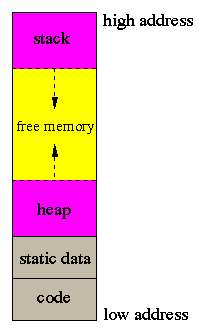
\includegraphics[width=0.2\textwidth]{memory_storage_management}
	%\caption{Manejo de stack y heap}
	\label{fig:memory_storage_management}
\end{figure}

This is the layout in memory of an executable program. Note that in a virtual memory architecture (which is the case for any modern operating system), some parts of the memory layout may in fact be located on disk blocks and they are retrieved in memory by demand (lazily).

The machine code of the program is typically located at the lowest part of the layout. Then, after the code, there is a section to keep all the fixed size static data in the program. The dynamically allocated data (ie. the data created using malloc in C) as well as the static data without a fixed size (such as arrays of variable size) are created and kept in the heap. The heap grows from low to high addresses. When you call malloc in C to create a dynamically allocated structure, the program tries to find an empty place in the heap with sufficient space to insert the new data; if it can't do that, it puts the data at the end of the heap and increases the heap size.

The focus of this section is the stack in the memory layout. It is called the run-time stack. The stack, in contrast to the heap, grows in the opposite direction (upside-down): from high to low addresses, which is a bit counterintuitive. The stack is not only used to push the return address when a function is called, but it is also used for allocating some of the local variables of a function during the function call, as well as for some bookkeeping.

Let’s consider the lifetime of a function call. When you call a function you not only want to access its parameters, but you may also want to access the variables local to the function. Worse, in a nested scoped system where nested function definitions are allowed, you may want to access the local variables of an enclosing function. In addition, when a function calls another function, we must forget about the variables of the caller function and work with the variables of the callee function and when we return from the callee, we want to switch back to the caller variables. That is, function calls behave in a stack-like manner.

El Stack mantiene el Registro de Activación o frame. A call stack is composed of stack frames (also called activation records or activation frames). These are machine dependent and ABI-dependent data structures containing subroutine state information. Each stack frame corresponds to a call to a subroutine which has not yet terminated with a return.
El \emph{stack frame} usualmente incluye al menos los siguientes items (en orden en que se encolan):
\begin{itemize}
	\item Argumentos (parámetros) pasados a la rutina (si posee alguno)
	\item Dirección de retorno a la rutina invocadora (ej. En el stack frame de una función \texttt{DibujarLinea}, una dirección al código de la función que la llamó, como puede ser \texttt{DibujarCuadrado})
	\item Espacio para las variables locales de la rutina (si existen).
\end{itemize}

Para el procesador es difícil manejar la memoria: no toda la memoria es igual.

El uso de la memoria cache no depende del programador ni del sistema operativo. Sólo la ve el hardware (la microarquitectura).

A CPU cache is a cache used by the central processing unit (CPU) of a computer to reduce the average time to access data from the main memory. The cache is a smaller, faster memory which stores copies of the data from frequently used main memory locations. Most CPUs have different independent caches, including instruction and data caches, where the data cache is usually organized as a hierarchy of more cache levels (L1, L2 etc.)

\subsubsection{Ciclo de instruccion}
An instruction cycle (sometimes called fetch-and-execute cycle, fetch-decode-execute cycle, or FDX) is the basic operation cycle of a computer. It is the process by which a computer retrieves a program instruction from its memory, determines what actions the instruction requires, and carries out those actions. This cycle is repeated continuously by the central processing unit (CPU), from bootup to when the computer is shut down.

\subsection{Modos de direccionamiento}
\subsubsection{Modos de direccionamiento para código}
El compilador genera las direcciones de las instrucciones:
\begin{itemize}
	\item Puede ser una dirección absoluta $\Rightarrow$ secuencial.
	\item Puede ser relativa al Program Counter (position independent) $\Rightarrow$ secuencial
	\item Puede generar las direcciones en cada instrucción como SECD para cálculo
\end{itemize}

\subsubsection{Modos de direccionamiento para datos}
\begin{itemize}
	\item Dirección Absoluta
	\item Operador Inmediato (literal)
	\item Dirección indirecta (*ptr)
	\item Dirección relativa a Program Counter (*+ptr)
	\item Base/Índice/Offset.
	\item Base + Desplazamiento
\end{itemize}

\subsection{Protección de memoria}
El Sistema Operativo debe impedir a un proceso invadir la memoria de otro.

Un espacio de direcciones es un set de direcciones que un proceso puede usar para direccionar memoria. Cada proceso tiene su propio set de direcciones, independiente de aquellos que pertenecen a otro proceso.

Una forma de hacerlo es por medio de un \emph{registro base} y uno \emph{límite}. El registro base puede usarse para direccionamiento indirecto. Cada dirección se compara con ambos límites.

El Sistema Operativo no tiene restricciones al operar en Modo Kernel

\begin{figure}[H]
	\centering
	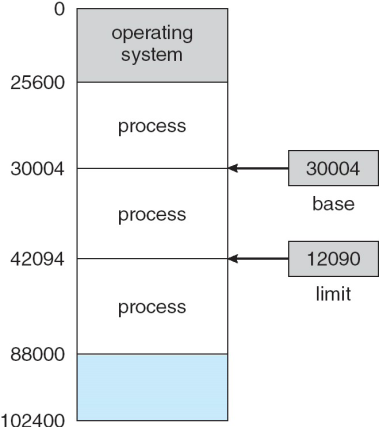
\includegraphics[width=0.2\textwidth]{memory_protection}
	%\caption{Protección por espacios de memoria}
	\label{fig:memory_protection}
\end{figure}

\subsection{Administración de memoria por el sistema operativo}
El Modelo de Procesos añade un área especial para la administración del proceso (La U\_Area).

El Sistema Operativo debe proveer alojamiento para la ejecución del proceso (Memory Allocation).

En multiprocesamiento, más de un proceso hace sus requerimientos de memoria.

\subsubsection{Segmentación}
\begin{itemize}
	\item Es una forma de proveer de más de un espacio de direcciones.
	\item El programador (o el compilador) es quien lo usa.
	\item Su uso puede superponerse con el del paginado.
	\item La protección puede asociarse a segmentos.
	\item Algunos sistemas separan las tablas de segmentos (ej. Intel):
	\begin{itemize}
		\item Global (para el Sistema Operativo)
		\item Local (para los procesos). O hasta una por proceso.
	\end{itemize}
\end{itemize}
Esto permite que los procesos no compitan con el Sistema Operativo por memoria.

\subsection{Administración del espacio libre/ocupado}
Memory allocation is the process of assigning blocks of memory on request. Typically the allocator receives memory from the operating system in a small number of large blocks that it must divide up to satisfy the requests for smaller blocks. It must also make any returned blocks available for reuse. There are many common ways to perform this, with different strengths and weaknesses.

Pueden usarse bitmaps o listas encadenadas. Aparecen distintos Algoritmos de alojamiento: \emph{Best Fit}, \emph{Worst Fit}, \emph{First Fit}, \emph{BuddySystem}, \emph{Swapping}.

\subsubsection{Best fit}
Buscar el hueco mas ajustado.

The allocator keeps a list of free blocks (known as the free list) and, on receiving a request for memory, scans along the list for the first block that is large enough to satisfy the request. If the chosen block is significantly larger than that requested, then it is usually split, and the remainder added to the list as another free block. The first fit algorithm performs reasonably well, as it ensures that allocations are quick.

\subsubsection{Worst fit}
Buscar el hueco más holgado.

This approach encourages external fragmentation, but allocation is very fast.

\subsubsection{First fit}
Buscar el primer hueco en que quepa.

The free block with the “tightest fit” is always chosen. The fit is usually sufficiently tight that the remainder of the block is unusably small.

Tienen rendimientos parecidos, pero generalmente First Fit funciona un poco mejor.

\subsubsection{Buddy system} 
Usado en los dispositivos modernos que no tienen memoria virtual (la memoria física es la que ven los procesos). 
La memoria se asigna en cantidades potencias de dos.

Permite una recuperación rápida de huecos grandes. Sufre de fragmentación interna. Su implementación es muy sencilla y rápida.

No se usa en SO de uso general.

In a buddy system, the allocator will only allocate blocks of certain sizes, and has many free lists, one for each permitted size. The permitted sizes are usually either powers of two, or form a Fibonacci sequence (see below for example), such that any block except the smallest can be divided into two smaller blocks of permitted sizes.
When the allocator receives a request for memory, it rounds the requested size up to a permitted size, and returns the first block from that size’s free list. If the free list for that size is empty, the allocator splits a block from a larger size and returns one of the pieces, adding the other to the appropriate free list.

When blocks are recycled, there may be some attempt to merge adjacent blocks into ones of a larger permitted size (coalescence). To make this easier, the free lists may be stored in order of address. The main advantage of the buddy system is that coalescence is cheap because the “buddy” of any free block can be calculated from its address.

\subsubsection{Swapping}
Consiste en pasar de memoria principal (RAM) a memoria secundaria (flash o disco rígido) un proceso que no está corriendo y que hace mucho que no está activado (ej: esperando intervención humana). Se baja todo el proceso. Pueden pasarse procesos bloqueados o disponibles pero sin ejecutarse.

Debe tenerse en cuenta la interacción con la I/O.

Se desplaza todo el proceso y se marca en el PCB (process control block). Lo decide el SO.

Se hace cuando no hay más memoria principal disponible. 

Al hacer swap-in, un proceso puede volver a una dirección distinta. El direccionamiento indirecto resuelve la reubicación.

\newpage
\section{Memoria virtual}
\subsection{Overlays}
Solución para correr programas demasiado grandes para la memoria disponible. Se comparten partes de memoria.
Reemplaza un bloque de código por otro.

El programador debe planificar el uso de \emph{overlays} según el uso de las rutinas del sistema.

Aún se usa en PDAs, Celulares y Embedded.

\begin{figure}[H]
	\centering
	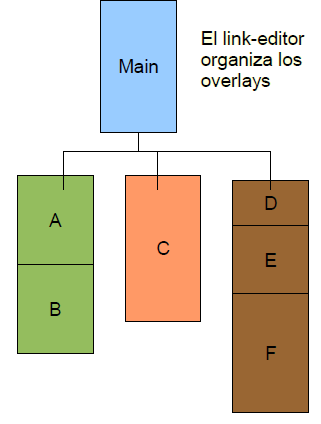
\includegraphics[width=0.2\textwidth]{virtual_memory_overlays}
	%\caption{Overlays}
	\label{fig:virtual_memory_overlays}
\end{figure}

Main puede llamar a cualquier procedimiento.
\textbf{A} puede llamar a \textbf{B}, pero no a \textbf{C} ni a \textbf{D}, \textbf{E} o \textbf{F}. \textbf{C} no puede llamar a ninguno.
Cada una de las tres partes son excluyentes

\subsection{Memoria virtual}
Evita que el programador deba planificar el uso de \emph{overlays}.

Básicamente, utilizando \emph{memoria virtual}, cada programa tiene su propio espacio de direcciones, que está fragmentado en bloques llamados \emph{páginas}. Cada página es un rango continuo de direcciones. Estas páginas están mapeadas en memoria física, pero no todas las páginas tienen que estar en memoria (física) para correr el programa.

Cuando el programa referencia una parte de su espacio de direcciones que está presente en memoria física, el hardware ejecuta el mapeo necesario al instante. En el caso que la parte no esté en memoria física, el sistema operativo es alertado para que busque la pieza faltante y reejecute la instrucción fallida.\\

Las principales ventajas de la memoria principal incluyen:
\begin{itemize}
	\item Liberar a las aplicaciones de tener que administrar un espacio de memoria compartido.
	\item Mejor seguridad debido al aislamiento de la memoria
	\item Poder ser capaz de, conceptualmente, utilizar más memoria que la disponible físicamente, utilizando la técnica de \emph{paginación}
\end{itemize}
Virtual memory makes application programming easier by hiding fragmentation of physical memory; by delegating to the kernel the burden of managing the memory hierarchy (eliminating the need for the program to handle overlays explicitly); and, when each process is run in its own dedicated address space, by obviating the need to relocate program code or to access memory with relative addressing.
Most virtual memory systems use a technique called paging.

\subsection{Páginas}
A page, memory page, or virtual page is a fixed-length contiguous block of virtual memory, described by a single entry in the page table. It is the smallest unit of data for memory allocation performed by the operating system on behalf of a program, and for transfers between the main memory and any other auxiliary store, such as a hard disk drive.

Virtual memory allows a page that does not currently reside in main memory to be addressed and used. If a program tries to access a location in such a page, an exception called a page fault is generated. The hardware or operating system is notified and loads the required page from the auxiliary store (hard disk) automatically. A program addressing the memory has no knowledge of a page fault or a process following it. Thus a program can address more (virtual) RAM than physically exists in the computer. Virtual memory is a scheme that gives users the illusion of working with a large block of contiguous memory space (perhaps even larger than real memory), when in actuality most of their work is on auxiliary storage (disk). Fixed-size blocks (pages) or variable-size blocks of the job are read into main memory as needed.

A transfer of pages between main memory and an auxiliary store, such as a hard disk drive, is referred to as paging.

Las direcciones generadas por la CPU se dividen bloques de tamaño fijo llamados páginas.

Estas direcciones se llaman direcciones virtuales.

Generalmente de 2 o 4 KB para evitar fragmentación interna.

Esta técnica permite el uso de memoria no contigua.

Las páginas se guardan en disco en un \emph{page data set}.

\subsection{Marcos de páginas (frames)}
La memoria principal se divide en frames, del mismo tamaño que las páginas.

Las direcciones de los frames se llaman direcciones reales.

Una unidad de Hardware, llamada \emph{MMU} (Memory Management Unit) mapea las direcciones virtuales en reales.

\subsubsection{Ejemplo de paging}
Generalmente las paginas y los frames son del mismo tamaño. Por ejemplo 4KB.

Si tenemos 64 KB de memoria virtual y 32 KB de memoria física, tenemos 16 páginas virtuales y 8 frames. De esta forma solo 8 páginas virtuales pueden estar mapeadas. Si el programa hace referencia a una pagina que no esta mapeada, el CPU hace un trap (\emph{page fault}) al SO, para reemplazar una pagina mapeada (poco usada) por la pagina nueva. Se escribe la pagina vieja en disco y se mapea la nueva.

\subsection{Page table}
Mapea las paginas con los frames.
\subsubsection{Estructura}
La estructura de una entrada en la tabla de paginación puede variar de maquina a maquina.
Ejemplo:
\begin{figure}[H]
	\centering
	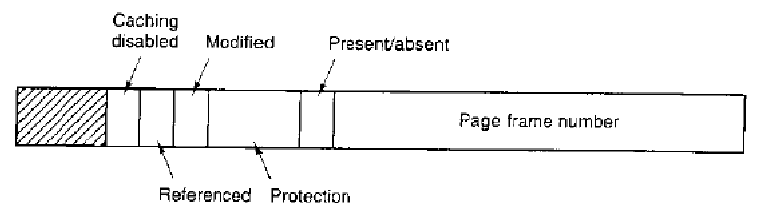
\includegraphics[width=0.6\textwidth]{virtual_memory_page_entry}
	%\caption{Entrada a la tabla de paginación}
	\label{fig:virtual_memory_page_entry}
\end{figure}

\begin{description}
	\item[Page frame number]
	\item[Present / absent bit] Si es 1, la entrada es válida y se puede usar. Si es 0, la pagina virtual no está actualmente en memoria. Acceder a una página cuyo bit está en 0 causa un page fault.
	\item[Protection bit] Dice que tipo de acceso tiene permitido (lectura, lectura/escritura).
	\item[Modified (“dirty") bit] cuando se escribe en una pagina, el hardware automáticamente setea el bit Modified en 1. Este bit se lee cuando el sistema operativo decide bajar esta página de memoria. Si la pagina fue modifica (es “dirty”), se debe guardar de vuelta en disco. Si no fue modificada (“clean”), se puede directamente abandonar, ya que la copia que está en disco es válida.
	\item[Referenced bit] Se setea cuando una pagina es referenciada, ya sea para lectura o escritura. Ayuda al sistema operativo a elegir que pagina dar de baja. Las páginas que no están siendo usadas son mejores candidatas a ser dadas de baja.
	\item[Caching] Se puede habilitar o deshabilitar el cacheo de la pagina.
\end{description}

\subsubsection{Tabla de páginas directa}
Se utiliza una \emph{tabla hash}, donde el valor del hash es el número de la página virtual. Cada entrada en la tabla hash contiene una lista enlazada de elemento que dirigen a la misma posición.

\subsubsection{Tabla de página multinivel}
Cuando crece mucho el espacio de memoria se usan tablas que referencias otras tablas y estas a su vez referencian a los frames como en el caso de paginación directo.

Se tiene en memoria las tablas que están siendo utilizadas y se deja en disco aquellas que no están siendo referenciadas.

\subsubsection{Tabla de página invertidas}
Es otra solución al problema del crecimiento del espacio de memoria.

En este diseño en vez de tener una tabla con cada espacio de memoria virtual referenciando su frame en memoria real es al revés.

La clave de la tabla es el frame, es decir que hay tantas entradas en la tabla como espacio de memoria real.

Se ahorra mucho espacio pero el cálculo de dirección es más costoso, para encontrar una dirección hay que iterar sobre la tabla buscando la dirección.

En la práctica el TBL guarda las páginas más utilizadas.

\subsection{Memory management unit (MMU)}
Es el responsable de traducir las direcciones virtuales (o lógicas) a direcciones reales (o físicas).
En general hace uso de una cache asociativo, el \emph{Translation Lookaside Buffer (TLB)}.

This solution is based on the observation that most programs tend to make a large number of references to a small number of pages, and not the other way around. Thus only a small fraction of the page table entries are heavily read; the rest are barely used at all.

The solution is a small hardware device for mapping virtual addresses to physical addresses without going through the page table. It is usually inside the MMU and consits of a small number of entries. Each entry contains information about one page, including the virtual page numbet, a bit that is set when the page is modified, the protection code (read/write/execute permissions), and the physical page frame in which the page is located. These fields have a one-to-one correspondence with the fields in the page table, except for the virtual page number, which is not needed in the page table. Another bit indicates wheter the entry is valid (i.e, in use) or not.

When a virtual address is presented to the MMU for translation, the hardware first checks to see if its virtual page number is present in the TLB by comparing it to all the entries simultaneously (in parallel). If a valid math is found, the page frame is taken directly from the TLB, without going to the page table.

If the virtual page number is not in the TLB, the MMU detects the miss and does an ordinary page table lookup. It then evicts one of the entries from the TLB and replaces it with the page table entry just looked up. Thus if that page is used again soon, the second time it will result in a TLB hit rather than a miss. When an entry is purged from the TLB, the modified bit is copied back into the page table entry in memory. The other values are already there, except the reference bit. When the TLB is loaded from the page table, all the fields are taken form memory.
Si no está el hardware en el \emph{MMU}, existen algunas soluciones para implementar el TLB con software.

\begin{description}
	\item[Hit/miss ratio] relación entre aciertos y fracasos.
	\item[Oportunidades de optimización] ~
	\begin{itemize}
		\item Algoritmos de paginado. 
		\item Que partes pasar al Hard.
		\item Como evitar los page faults.
		\item Estructura de las tablas de páginas.
		\item Organización del Page Data Set.
		\item Algunas otras cosas que se resuelven con el paginado.
	\end{itemize}
\end{description}

\subsection{Algoritmos de reemplazo de páginas}
\begin{enumerate}
	\item The theoretically optimal page replacement algorithm
	\item Not recently used
	\item FIFO
	\item Second-chance
	\item Clock
	\item Least recently used
	\item Random
	\item Not frequently used
	\item Aging
\end{enumerate}

\subsubsection{The theoretically optimal page replacement algorithm}
The theoretically optimal page replacement algorithm is an algorithm that works as follows: when a page needs to be swapped in, the operating system swaps out the page whose next use will occur farthest in the future.

This algorithm cannot be implemented in the general purpose operating system because it is impossible to compute reliably how long it will be before a page is going to be used, except when all software that will run on a system is either known beforehand and is amenable to the static analysis of its memory reference patterns, or only a class of applications allowing run-time analysis.

\subsubsection{Not recently used}
The not recently used (NRU) page replacement algorithm is an algorithm that favours keeping pages in memory that have been recently used. This algorithm works on the following principle: when a page is referenced, a referenced bit is set for that page, marking it as referenced. Similarly, when a page is modified (written to), a modified bit is set. The setting of the bits is usually done by the hardware, although it is possible to do so on the software level as well.

At a certain fixed time interval, the clock interrupt triggers and clears the referenced bit of all the pages, so only pages referenced within the current clock interval are marked with a referenced bit. When a page needs to be replaced, the operating system divides the pages into four classes:
\begin{description}
	\item[3] referenced, modified
	\item[2] referenced, not modified
	\item[1] not referenced, modified
	\item[0] not referenced, not modified
\end{description}

Although it does not seem possible for a page to be not referenced yet modified, this happens when a class 3 page has its referenced bit cleared by the clock interrupt. The NRU algorithm picks a random page from the lowest category for removal. So out of the above four pages, the NRU algorithm will replace the not referenced, not modified. Note that this algorithm implies that a modified but not referenced (within last clock interval) page is less important than a not modified page that is intensely referenced.

\subsubsection{FIFO}
Requiere mantener una cola de páginas.

No es buena idea.

Reemplaza las páginas del scheduler o del Kernel.

Este algoritmo experimenta la anomalía de Belady (the phenomenon where increasing the number of page frames results in an increase in the number of page faults for a given memory access pattern)

\subsubsection{Second-chance}
A modified form of the FIFO page replacement algorithm, known as the Second-chance page replacement algorithm, fares relatively better than FIFO at little cost for the improvement. It works by looking at the front of the queue as FIFO does, but instead of immediately paging out that page, it checks to see if its referenced bit is set. If it is not set, the page is swapped out. Otherwise, the referenced bit is cleared, the page is inserted at the back of the queue (as if it were a new page) and this process is repeated. This can also be thought of as a circular queue. If all the pages have their referenced bit set, on the second encounter of the first page in the list, that page will be swapped out, as it now has its referenced bit cleared. If all the pages have their reference bit set then second chance algorithm degenerates into pure FIFO.

As its name suggests, Second-chance gives every page a ``second-chance'' – an old page that has been referenced is probably in use, and should not be swapped out over a new page that has not been referenced.

\subsubsection{Clock}
Clock is a more efficient version of FIFO than Second-chance because pages don't have to be constantly pushed to the back of the list, but it performs the same general function as Second-Chance. The clock algorithm keeps a circular list of pages in memory, with the ``hand'' (iterator) pointing to the last examined page frame in the list. When a page fault occurs and no empty frames exist, then the R (referenced) bit is inspected at the hand's location. If R is 0, the new page is put in place of the page the ``hand'' points to, otherwise the R bit is cleared. Then, the clock hand is incremented and the process is repeated until a page is replaced.

\subsubsection{Least recently used}
Cada referencia a memoria actualiza un timestamp en la page table. Se reemplaza la página cuyo time stamp sea el más antiguo. Requiere bastante auxilio de hard para tener una performance adecuada.

\subsubsection{Random}
Random replacement algorithm replaces a random page in memory. This eliminates the overhead cost of tracking page references. Usually it fares better than FIFO, and for looping memory references it is better than LRU, although generally LRU performs better in practice.

\subsubsection{Not frequently used}
The not frequently used (NFU) page replacement algorithm requires a counter, and every page has one counter of its own which is initially set to 0. At each clock interval, all pages that have been referenced within that interval will have their counter incremented by 1. In effect, the counters keep track of how frequently a page has been used. Thus, the page with the lowest counter can be swapped out when necessary.

Problema: No tiene en cuenta el tiempo. Nunca olvida!

\subsubsection{Aging}
The aging algorithm is a descendant of the NFU algorithm, with modifications to make it aware of the time span of use. También tiene un contador, por cada referencia se enciende el primer bit. Cuando se produce una interrupción de reloj (~ 0,02 s), el SO desplaza todos los bits una posición a la derecha. Cuando ocurre un fallo se cambia la página de menor valor en el contador.

\subsection{Otros conceptos}
\subsubsection{Working set}
Los programas exhiben un comportamiento conocido como localidad de referencia. En cada fase de su ejecución, el proceso referencia solo a un pequeño número de páginas (no necesariamente contiguas). Ese conjunto se llama Working Set (aunque la definición cambia con la implementación). El Working Set va cambiando a medida que progresa la ejecución.

\subsubsection{Pre-paginado}
Si un proceso pagina durante mas tiempo que el que ejecuta se dice que hace thrashing. This leads to low CPU utilization.

Posible solución: Se pre-pagina (cargan en memoria) todas las páginas del último Working Set del proceso. Se re-calcula el Working Set a intervalos.

\subsubsection{Tablas de páginas Locales y Globales}
Algunos Sistemas permiten el reemplazo de cualquier página (paginado global).

Otros solo permiten que un proceso pagine sobre si mismo, evitando efectos en la performance del resto. Esta estrategia es la que se usaría en un Sistema Operativo orientado a Objetos.

En general, el paginado global funciona mejor. Ya que no todos los procesos tienen los mismos requerimientos.

\subsubsection{Archivos de paginado}
Una página no es una buena unidad de transferencia.

Se usan entonces láminas (slab) de páginas en cada transferencia. La ubicación de una página es entonces \#slab + offset. Las slabs se acomodan en el page data set (o partición de paginado). Que se formatea y ubica por anticipado.

\subsubsection{Paginado de código}
Las páginas de código son read-only.

Se paginan directamente desde el archivo del programa ejecutable.

El elf tiene previsiones para ello.

Es una forma muy eficiente de cargar un programa a memoria. El resto de las páginas tiene su ``shadow'' en disco.

\subsubsection{Otros tópicos}
El paginado interactúa con la I/O. Se deben fijar las páginas donde hay transferencia desde memoria secundaria. Los archivos pueden accederse como memoria virtual.

\newpage
\section{Linkers y loaders}
\subsection{Linker}
\subsubsection{Definición}
Un \emph{linker} o \emph{link editor} es un programa que toma uno o más \emph{archivos objeto} generados por un compilador y los combina en un único archivo ejecutable, o en un archivo objeto más.

Un archivo objeto es un archivo que contiene \emph{código objeto}, es decir, código de máquina reacomodable que usualmente no se puede ejecutar directamente. Los archivo objeto son producidos por un \emph{ensamblador}, \emph{compilador} u otro traductor de lenguajes.

\begin{center}
	Programa fuente (1 o varios) $\Rightarrow$ Traductor $\Rightarrow$ Programa objeto (1 o varios)
\end{center}

\subsubsection{Traducción - ensamblado}
\begin{itemize}
	\item Si el lenguaje es un assembler, la traducción es un ensamblado (assembly) hecho por un programa ensamblador (assembler).
	\item Convierte código de lenguaje ensamblador memotécnico a códigos de operación (machine language instruction).
	\item Resuelve identificadores a posiciones de memoria.
	\item Algunos proveen abstracciones de programación avanzadas.
Existe un assembler distinto para cada arquitectura, incluso hay assemblers generales.
\end{itemize}

\subsubsection{Traducción - compilación}
Si se trata de un lenguaje de alto o mediano nivel, la traducción es una compilación.

\begin{center}
	Lenguaje fuente $\Rightarrow$ Traductor (compilador) $\Rightarrow$ Lenguaje objeto (.o) (microarquitectura)
\end{center}

\subsubsection{Link-editor}
\begin{description}
	\item[Entradas] ~
	\begin{itemize}
		\item Programas objeto
		\item Bibliotecas
		\item Programas ejecutables: para usarlas como apis. No recomendable.
	\end{itemize}

	\item[Salidas] ~
	\begin{itemize}
		\item Programas ejecutables
		\item Programas objeto
		\item Bibliotecas
	\end{itemize}
\end{description}

\textbf{Mezcla las direcciones de cada módulo en un único espacio de direcciones.}

Biblioteca y programa objeto no ejecutable son diferentes conceptualmente (de objetivos de creación):
La biblioteca es pensada para usarse en diferentes programas, mientras que el programa objeto se crea para un programa en particular.

\begin{figure}[H]
	\centering
	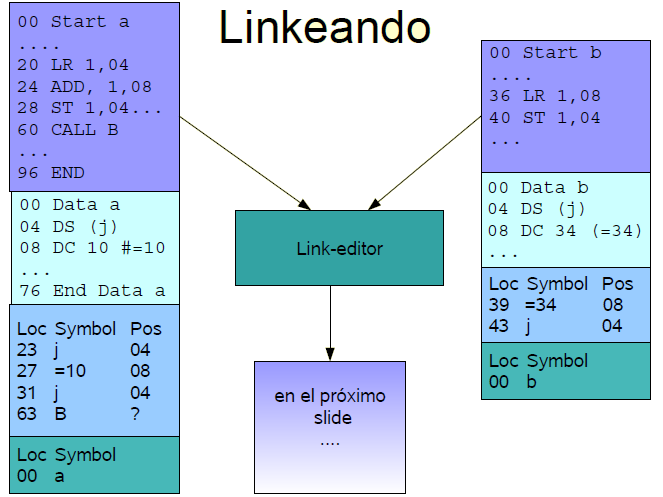
\includegraphics[width=0.6\textwidth]{linkers_loaders_linking_1}
	%\caption{---}
	\label{fig:linkers_loaders_linking_1}
\end{figure}

\begin{figure}[H]
	\centering
	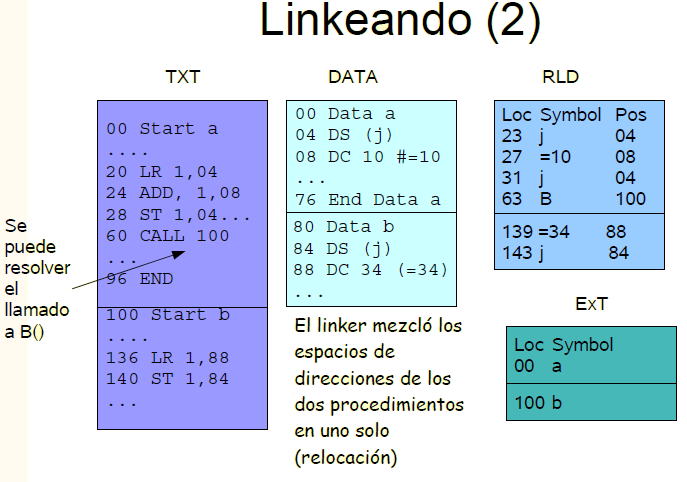
\includegraphics[width=0.6\textwidth]{linkers_loaders_linking_2}
	%\caption{---}
	\label{fig:linkers_loaders_linking_2}
\end{figure}

\subsection{Loader}
En el linker, el ejecutable puede incluir las bibliotecas o no
\begin{itemize}
	\item Si lo incluye (forma \emph{estática}), el programa ya incluye los símbolos y están cargados en memoria.
	\item Si no se incluyen, las llamadas a la biblioteca se resuelven en tiempo de ejecución (forma \emph{dinámica}). El \textbf{loader} vincula las llamadas con la biblioteca.
\end{itemize}
	
Permite cambiar el funcionamiento actualizando las librerías del SO. Pero depende de que la biblioteca exista en el SO, y existen problemas de seguridad por ejecutar el código externo.

Linker y loader son en momento de post-compilación.

\begin{figure}[H]
	\centering
	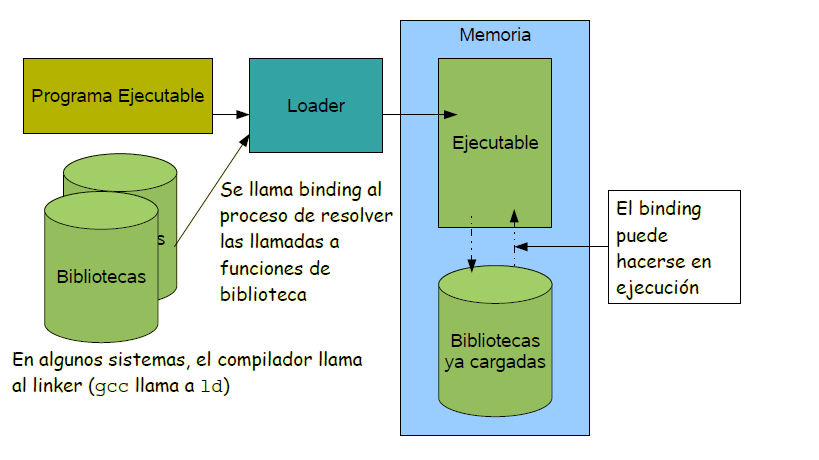
\includegraphics[width=0.7\textwidth]{linkers_loaders_loading_1}
	%\caption{---}
	\label{fig:linkers_loaders_loading_1}
\end{figure}

\begin{figure}[H]
	\centering
	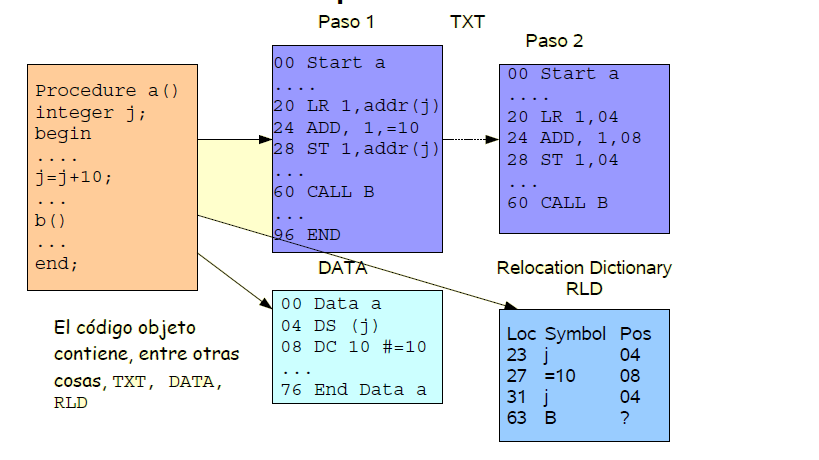
\includegraphics[width=0.7\textwidth]{linkers_loaders_loading_2}
	%\caption{---}
	\label{fig:linkers_loaders_loading_2}
\end{figure}

\begin{figure}[H]
	\centering
	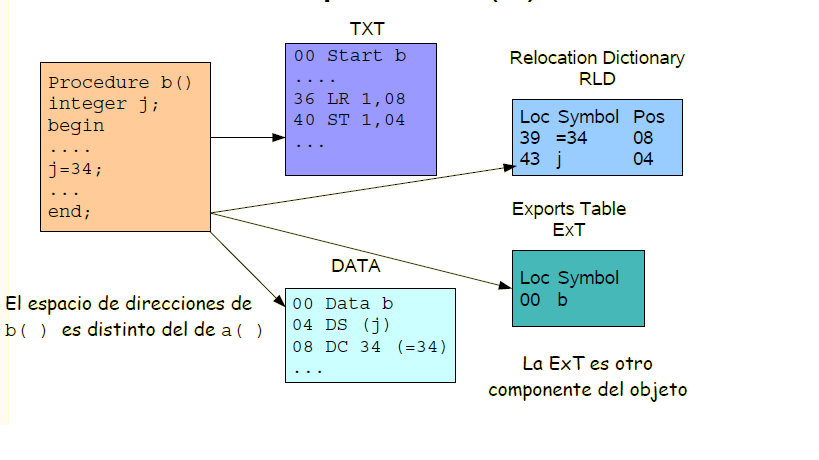
\includegraphics[width=0.7\textwidth]{linkers_loaders_loading_3}
	%\caption{---}
	\label{fig:linkers_loaders_loading_3}
\end{figure}

\subsection{Object file formats (OFF)}
Es clave para la performance del sistema.

Algunos prevén su interacción con el paginado.

Se suele utilizar el mismo formato para ejecutables, objetos y bibliotecas.

Que dos Sistemas Operativos tengan el mismo OFF no significa que los programas de uno puedan correr en el otro.
\begin{description}
	\item[com] ~
	\begin{itemize}
		\item Se usan en DOS.
		\item Son los que tienen extensión .com. Microsoft los llama bin o binary file
		\item Se cargan en una dirección fija de memoria (0x100).
		\item Datos y código están en el mismo segmento.
		\item Son monousuario y monoproceso
	\end{itemize}

	\item[exe] ~
	\begin{itemize}
		\item Aparece en DOS 2.0.
		\item Su primer byte o (Magic Number) es “MZ”, iniciales de Mark Zbikowski.
		\item Tiene previsión para relocación en memoria.
	\end{itemize}

	\item[Common Object File Format (COFF)] ~
	\begin{itemize}
		\item Aparece en Unix pero se usa en otros ambientes.
		\item Se compone de varias secciones separadas por headers (con limitación de longitud).
		\item Se usa para bibliotecas (Aunque no de enlace dinámico).
		\item Soporta debug (pero solo de C): nm(1) lo puede inspeccionar.
	\end{itemize}

	\item[Windows Portable Executable (PE)] ~
	\begin{itemize}
		\item Es una adaptación del COFF. El Windows hace un wrapping del COFF.
		\item Su magic es “PE” pero comienza con un “MZ” por “compatibilidad”.
		\item Tiene definido espacio para resources.
		\item Tiene definido tablas para el uso de bibliotecas compartidas.
	\end{itemize}

	\item[Executable and Linkable Format (ELF)] ~
	
	Debido a su diseño, ELF es flexible y extensible, y no está atado a ningún procesador o arquitectura en particular. Esto le permitió ser adoptado por muchos sistemas operativos en distintas plataformas, convirtiéndolo en un estándar de facto.

	Cada ELF posee un ELF header, seguido de los datos del archivo. Estos datos pueden incluir:
	\begin{itemize}
		\item Program header table, describing zero or more segments
		\item Section header table, describing zero or more sections
		\item Data referred to by entries in the program header table or section header table
	\end{itemize}

	The segments contain information that is necessary for runtime execution of the file, while sections contain important data for linking and relocation. Any byte in the entire file can be owned by at most one section, and there can be orphan bytes, which are not owned by any section.

	El ELF header define si se utilizan direcciones de 32 o 64 bits.

	Sirve para ejecutables y bibliotecas.

	Un directorio permite agregar nuevas secciones.

	Tiene previsiones para emulación.

	\item[Binarios Universales] ~

	Tiene los códigos de las distintas arquitecturas y cuando se ejecuta decide cual usa.

	A fat binary (or multiarchitecture binary) is a computer executable program, which has been expanded (or ``fattened'') with code native to multiple instruction sets which can consequently be run on multiple processor types. The usual method of implementation is to include a version of the machine code for each instruction set, preceded by code compatible with all operating systems, which executes a jump to the appropriate section. This results in a file larger than a normal one-architecture binary file, thus the name.
\end{description}

\subsection{Segmentación de memoria en OFF}
Memory segmentation is the division of a computer's primary memory into segments or sections. In a computer system using segmentation, a reference to a memory location includes a value that identifies a segment and an offset within that segment. Segments or sections are also used in object files of compiled programs when they are linked together into a program image and when the image is loaded into memory.

Segments usually correspond to natural divisions of a program such as individual routines or data tables so segmentation is generally more visible to the programmer than paging alone. Different segments may be created for different program modules, or for different classes of memory usage such as code and data segments. Certain segments may be shared between programs.

\newpage
\section{Bibliotecas (Libraries)}
Las bibliotecas son una \emph{colección de subprogramas} usados en el desarrollo de Software.

Contienen ``código auxiliar'' y datos que brindan servicios a distintos programas.

Permiten el desarrollo modular.

Convierten los servicios en ``commodities'' entre los cuales se puede elegir.

The value of a library is the reuse of the behavior. When a program invokes a library, it gains the behavior implemented inside that library without having to implement that behavior itself. Libraries encourage the sharing of code in a modular fashion, and ease the distribution of the code.

\subsection{Tipos de bibliotecas}
Se clasifican según el tiempo en que se cargan al programa (y por ende la ubicación del código fuente y quien lo hace)
\begin{enumerate}
	\item Estáticas
	\item Dinámicas
	\item Dinámicas compartidas
\end{enumerate}

\subsubsection{Estáticas}
Los subprogramas se incluyen en el ejecutable. El link-editor es quien las incorpora al archivo ejecutable. Los símbolos quedan definidos.

\begin{description}
	\item[Ventajas] ~
	\begin{itemize}
		\item Facilitan la instalación de los programas en otras máquinas, ya que la aplicación queda contenida en un único archivo ejecutable.
		\item The application can be certain that all its libraries are present and that they are the correct version. This avoids dependency problems, known colloquially as DLL Hell or more generally dependency hell.
		\item Evitan que los troyanos ataquen programas sensibles (se sabe a exactamente qué código se esta corriendo, cosa que no pasa con las bibliotecas dinámicas).
		\item It is enough to include those parts of the library that are directly and indirectly referenced by the target executable (or target library). With dynamic libraries, the entire library is loaded, as it is not known in advance which functions will be invoked by applications. Whether this advantage is significant in practice depends on the structure of the library.
	\end{itemize}

	\item[Desventajas] ~
	\begin{itemize}
		\item In static linking, the size of the executable becomes greater than in dynamic linking, as the library code is stored within the executable rather than in separate files. But if library files are counted as part of the application then the total size will be similar.
	\end{itemize}
\end{description}


\subsubsection{Dinámicas}
El link-editor solo indica las llamadas. Éstas las resuelve el Loader durante la carga o durante la ejecución. Si es en ejecución, no carga la biblioteca cuando se ejecuta, sino cuando la necesita.\\

\begin{description}
	\item[Ventajas] ~
	\begin{itemize}
		\item Permite cambiar el funcionamiento actualizando las librerías del SO.
		\item Genera ejecutables más pequeños.
	\end{itemize}

	\item[Desventajas] ~
	\begin{itemize}
		\item Depende de que la biblioteca exista en el SO.
		\item Problemas de seguridad por ejecutar código externo.
	\end{itemize}
\end{description}

Se debe solucionar el problema de la \emph{relocación}: No se puede depender de posiciones ``absolutas'' de memoria ni en el programa ni en las bibliotecas. Se deben calcular las direcciones cada vez que se carga el programa o la biblioteca.

En general se usa una Import Table como acceso indirecto a las direcciones de la biblioteca para simplificar el proceso de linking.\\

\textbf{Relocación}

Relocation is the process of assigning load addresses to various parts of a program and adjusting the code and data in the program to reflect the assigned addresses. A linker usually performs relocation in conjunction with symbol resolution, the process of searching files and libraries to replace symbolic references or names of libraries with actual usable addresses in memory before running a program.

Relocation is typically done by the linker at link time, but it can also be done at run time by a relocating loader, or by the running program itself. Some architectures avoid relocation entirely by deferring address assignment to run time; this is known as zero address arithmetic.

Relocation is typically done in two steps:
\begin{enumerate}
	\item Each object file has various sections like code, data, .bss etc. To combine all the objects to a single executable, the linker merges all sections of similar type into a single section of that type. The linker then assigns run time addresses to each section and each symbol. At this point, the code (functions) and data (global variables) will have unique run time addresses.
	\item Each section refers to one or more symbols which should be modified so that they point to the correct run time addresses based on information stored in a relocation table in the object file.
\end{enumerate}

\subsubsection{Dinamicas Compartidas (DLL de windows)}
\begin{itemize}
	\item Están una sola vez en memoria. La comparten todos los procesos que la usan. 
	\item Se guardan en un PE.
	\item Pueden contener código, datos o recursos (iconos, menus, bitmaps, templates, fonts, etc).
	\item Proveen modularidad para desarrollo y mantenimiento.
\end{itemize}

\textbf{DLL Hell}

There are a number of problems commonly encountered with DLLs – especially after numerous applications have been installed and uninstalled on a system. The difficulties include conflicts between DLL versions, difficulty in obtaining required DLLs, and having many unnecessary DLL copies. As a result, an installation of a program that installs a new version of a common object may inadvertently break other programs that were previously installed.

The ambiguity with which DLLs that are not fully qualified can be loaded in the Windows operating system has been exploited by malware in recent years, opening a new class of vulnerability that affects applications from many different software vendors, as well as Windows itself.\\

\textbf{Funcionamiento}

En Win32 el archivo de las DLL está organizado en secciones:
\begin{itemize}
	\item Cada sección tiene sus propios atributos (ejecutable, compartible, solo lectura, etc).
	\begin{itemize}
		\item Generalmente hay una sola copia de las secciones de código en memoria (se comparte).
		\item En cambio las secciones de datos son privadas (aunque pueden compartirse).
	\end{itemize}
	\item Las bibliotecas comprimidas (con UPX por ejemplo) permanecen privadas.
	\item Los símbolos exportados tienen como identificador un número y un nombre.
	\begin{itemize}
		\item Solo los nombres se mantienen entre distintas versiones.
		\item Se puede hacer un bind a una rutina de una versión específica.
	\end{itemize}
\end{itemize}

\textbf{El linkeo puede ser}
\begin{enumerate}
	\item \textbf{Load-time dynamic linking:} El linking se hace al cargar el programa. El programador no tiene control si no se encuentra la DLL
	\item \textbf{Run time dynamic linking:} Se hace por medio de un llamado a \texttt{LoadLibrary()}. El programador puede intervenir si hay error.
\end{enumerate}

Para saber que bibliotecas se usan, hay programas como Dependency Walker.\\

\textbf{Bibliotecas en Linux}
Las bibliotecas comienzan con lib. Las de enlace estático terminan en .a y las de enlace dinámico en .so. Por ejemplo la biblioteca foo es libfoo.a y dynfoo es libdynfoo.so.

Además se agrega un número de versión.

Las dependencias se ven con ldd.\\

\textbf{Position Independent Code (PIC o PIE)}

Es código que puede ejecutar correctamente en forma independiente de su posición en la memoria.

PIC is commonly used for shared libraries, so that the same library code can be loaded in a location in each program address space where it will not overlap any other uses of memory (for example, other shared libraries).

Position-independent code can be executed at any memory address without modification. This differs from relocatable code, where a link editor or program loader modifies a program before execution, so that it can be run only from a particular memory location. Position-independent code must adhere to a specific set of semantics in the source code and compiler support is required. Instructions that refer to specific memory addresses, such as absolute branches, must be replaced with equivalent program counter relative instructions.

Las DLL de Windows no son PIE ni PIC.\\

\textbf{Run Time Linking en Linux}

Se hace por medio de la interface de programador del linker dinámico: \texttt{dlopen()}, \texttt{dlsym()}, \texttt{dlclose()}, \texttt{dlerror()}.

\newpage
\section{Virtualización}
Llamamos virtualización a la abstracción de recursos de computación
\begin{itemize}
	\item Virtualización de Aplicaciones.
	\item Virtualización de Plataforma.
	\item Virtualización de Escritorio.
	\item Virtualización de recursos: Red, Memoria, Almacenamiento, clusters, grids.
\end{itemize}

\begin{description}
	\item[Objetivos] Permite compartimentar la ejecución de varias aplicaciones en el mismo servidor, de manera independiente y transparente. Independiza la ejecución de la capa física.

	\item[Ventajas] ~
	\begin{itemize}
		\item \textbf{Aumento de confiabilidad} Si una maquina que alberga muchos servicios se cae, se ven afectados todos. En cambio, si cada servicio está en maquinas distintas, sólo se ve afectado uno. Una maquina física puede tener varias maquinas virtuales (es mas barato que varias maquinas físicas). Sirve porque es (mucho) más común que falle una maquina debido al software que al hardware.
		\item \textbf{Aplicaciones antiguas (legacy)}
		\item \textbf{Desarrollo y prueba en múltiples plataformas}
		\item \textbf{Balanceo de cargas y escalabilidad futura} Es mas fácil migrar de una VM a otra en un host demasiado cargado.	
	\end{itemize}
\end{description}

\subsection{Virtualización de aplicaciones}
Compatibilidad y portabilidad entre distintos Sistemas Operativos y distintas arquitecturas.

Application virtualization is software technology that encapsulates application software from the underlying operating system on which it is executed. A fully virtualized application is not installed in the traditional sense, although it is still executed as if it were. The application behaves at runtime like it is directly interfacing with the original operating system and all the resources managed by it, but can be isolated or sandboxed to varying degrees.

\begin{description}
	\item[Ventajas] ~
	\begin{itemize}
		\item Allows applications to run in environments that do not suit the native application
		\item May protect the operating system and other applications
		\item Uses fewer resources than a separate virtual machine (virtualización de plataforma)
	\end{itemize}

	\item[Ejemplos] ~
	\begin{itemize}
		\item Máquinas Virtuales (JVM, .net CLR)
		\item Compatibility Layers
	\end{itemize}
\end{description}

\subsection{Virtualización de plataformas}
Abstracción de todos los recursos de computación de un huésped dentro de un anfitrión (host). Computer hardware virtualization is the virtualization of computers or operating systems. It hides the physical characteristics of a computing platform from users, instead showing another abstract computing platform. Hace como si fuera otra plataforma en su totalidad.

\begin{description}
	\item[Tipos de virtualización] ~
	\begin{itemize}
		\item Virtualización total
		\begin{itemize}
			\item Emulación de plataforma.
			\item Hipervisores
		\end{itemize}
		\item Paravirtualización.
		\item Virtualización del mismo Sistema Operativo.
	\end{itemize}
\end{description}

\subsection{Condiciones para virtualizar}
\begin{description}
	\item[Instrucciones privilegiadas] Las que ocasionan un software trap.
	\item[Instrucciones delicadas (``sensitive'')] Las que solo pueden ejecutarse en Modo Supervisor del procesador porque afectan a los recursos del sistema, como I/O o cambios en la configuración del MMU.
\end{description}

\subsubsection{Teorema de Popek y Goldberg sobre virtualización}
Una arquitectura es virtualizable si las instrucciones delicadas son un subconjunto de las privilegiadas. Es decir, si en modo usuario tratar de hacer algo que no deberías poder hacer en modo usuario, debería llamarse un software trap.

\subsubsection{Virtualización de la IA32 (x86 virtualization)}
x86 tiene 17 instrucciones sensibles que no son privilegiadas, violando una de las condiciones de Popeck por lo que no es virtualizable en estas condiciones.

Para realizar la virtualización de esta máquina se requiere de una extensión que la permita, que en este caso es el Intel IVT, que genera containers en los que la ejecución de una instrucción sensible provoca un software trap. Luego, con la trampa se debe emular el comportamiento de la máquina autónoma del sistema operativo guest.

\subsection{Hipervisores}
Hipervisor es una pieza de software firmware o hardware que crea y ejecuta máquinas virtuales.

Una computadora en la cuál un hipervisor está ejecutando una o más máquinas virtuales es una maquina ``host''. Cada máquina virtual es llamada ``guest''.

El hipervisor se encarga de la ejecución del sistema operativo del guest, el cuál no sabe que está siendo ejecutado sobre una máquina virtual. Quien está consciente de esto es el hipervisor.

\subsubsection{Hipervisor tipo I}
\textbf{Corren directamente sobre el hardware}, el huésped debe tener una arquitectura virtualizable.

El huésped corre en modo usuario, su Kernel cree haber pasado a modo supervisor, pero continúa en modo usuario.
Cuando el sistema operativo guest ejecuta una instrucción sensible ocurre una ``kernel trap''.

Tiene que ser virtualizable según Popek y Goldberg.

\begin{figure}[H]
	\centering
	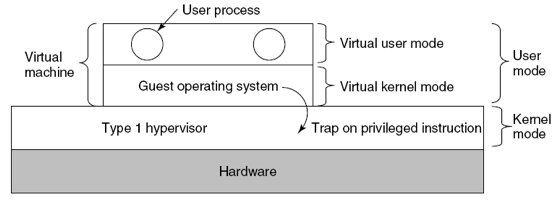
\includegraphics[width=0.7\textwidth]{\imgdir/virtualization_hipervisor_type_i}
	%\caption{-}
	\label{fig:virtualizacion_hipervisor_tipo_i}
\end{figure}

\subsubsection{Hipervisor tipo II}
Corre bajo el control de un sistema operativo anfitrión o host. 

Puede virtualizar cualquier ambiente, aún cuando éste no sea virtualizable según las condiciones de Popek y Goldberg.

\begin{figure}[H]
	\centering
	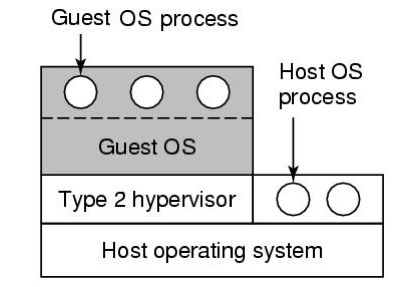
\includegraphics[width=0.5\textwidth]{\imgdir/virtualization_hipervisor_type_ii}
	%\caption{-}
	\label{fig:virtualizacion_hipervisor_tipo_ii}
\end{figure}

\subsubsection{Paravirtualización}
Paravirtualizar consiste en reemplazar, en el sistema operativo guest, las instrucciones delicadas por llamadas al hipervisor. En este caso, el sistema operativo huésped debe ser modificado para saber que va a correr en un entorno virtualizado. El huésped utiliza una API especial para comunicarse con la capa de virtualización e interactuar directamente con el hard. Si bien tenemos claros beneficios por el lado de la performance, se pierde compatibilidad ya que el SO huésped debe ser modificado. Requiere código fuente.

\textbf{La paravirtualización es distinta del hipervisor tipo II}

\begin{figure}[H]
	\centering
	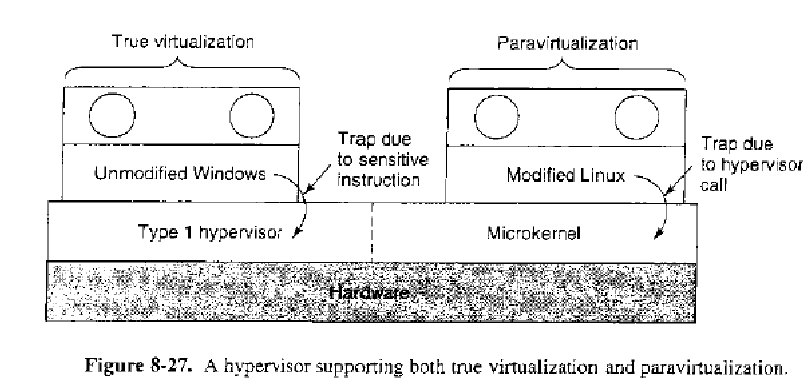
\includegraphics[width=0.7\textwidth]{\imgdir/virtualization_paravirtualization}
	%\caption{-}
	\label{fig:virtualizacion_paravirtualization}
\end{figure}

\subsubsection{Traducción binaria}
\textit{En tiempo de ejecución cambia las instrucciones sensibles por llamados a procedimientos de VM, es decir modifica la ejecución del programa.}\\

Traducción binaria, en cambio, consiste en examinar bloques básicos (código con un punto de entrada, uno de salida y sin jumps).

El Hipervisor modifica de esta forma el programa que está corriendo. Cuando va a ejecutar un programa, la VM primero examina el código buscando instrucciones sensibles, y las reemplaza por llamados a procedimientos de VM que las manejan.

El Hipervisor toma el control: Si la trap proviene del kernel del guest, lleva a cabo la acción correspondiente, si en cambio proviene de un programa en modo usuario, responde como lo haría el Hard.
Guarda el código traducido en el cache, para mejorar la performance.

Esto genera más sobrecarga que el enfoque de paravirtualización, pero no limita a usar sólo SO modificados, podemos usar cualquier SO. No requiere código fuente.

\subsection{Virtualización del Escritorio}
Las aplicaciones se hospedan en un sistema central pero cada usuario tiene su escritorio local.

Desktop virtualization is software technology that separates the desktop environment and associated application software from the physical client device that is used to access it.

Desktop virtualization can be used in conjunction with application virtualization and (Windows) user profile management systems, now termed ``user virtualization'', to provide a comprehensive desktop environment management system. In this mode, all the components of the desktop are virtualized, which allows for a highly flexible and much more secure desktop delivery model. In addition, this approach supports a more complete desktop disaster recovery strategy as all components are essentially saved in the data center and backed up through traditional redundant maintenance systems. If a user's device or hardware is lost, the restore is much more straightforward and simple, because basically all the components will be present at login from another device. In addition, because no data is saved to the user's device, if that device is lost, there is much less chance that any critical data can be retrieved and compromised. 

\subsection{Virtualización de recursos}
Usar los recursos del sistema operativo host para apoyar la ejecución del guest.

\subsection{Virtualización del Sistema Operativo}
Operating system–level virtualization is a server virtualization method where the kernel of an operating system allows for multiple isolated user space instances, instead of just one. Such instances (often called containers, virtualization engines (VE), virtual private servers (VPS) or jails) may look and feel like a real server from the point of view of its owners and users.

Cuando el Kernel permite distintos ambientes de usuarios aislados entre sí.

Usado por seguridad en aplicaciones como hosting virtual.

Virtual hosting environments commonly use operating system–level virtualization, where it is useful for securely allocating finite hardware resources amongst a large number of mutually-distrusting users. System administrators may also use it, to a lesser extent, for consolidating server hardware by moving services on separate hosts into containers on the one server.

Other typical scenarios include separating several applications to separate containers for improved security, hardware independence, and added resource management features. The improved security provided by the use of a chroot mechanism, however, is nowhere near ironclad.

OS-level virtualization implementations that are capable of live migration can be used for dynamic load balancing of containers between nodes in a cluster.

\newpage
\section{Archivos}
We have three essential requirements for long-term information storage:
\begin{itemize}
	\item It must be possible to store a very large amount of information (larger than the address space).
	\item The information must survive the termination of the process using it.
	\item Multiple processes must be able to access the information concurrently.
\end{itemize}

\subsection{Archivos}
Una colección de datos con nombre.

Una unidad lógica de almacenamiento. Abstrae las propiedades físicas del dispositivo de almacenamiento.

Provee persistencia a través de reinicios, activaciones de programas o fallas de energía.\\

\subsubsection{Atributos de un archivo}
\begin{description}
	\item[Nombre] When a process creates a file, it gives the file a name. When the process terminates, the file continues to exist and can be accessed by other processes usign its name. Distintos sistemas operativos tienen distintas restricciones respecto del largo, caracteres permitidos y case sensitivity
	
	\item[Ubicación] Punto de entrada del archivo (puede estar repartido).

	\item[Tipo] Restringe las operaciones que se pueden realizar sobre el archivo. Qué aplicaciones entienden al archivo.

	\textbf{Regular files} are the ones that contain user information. \textbf{Directories} are system files for maintaining the structure of the file system. \textbf{Character special files} are related to input/output and used to model serial I/O devices, such as terminals, printers and networks. \textbf{Block special files} are used to model disks.

	Regular files are generally ASCII files or binary files. 

	ASCII files consist of lines of text. The great advantage is that they can be displayed and printed as is, and they can be edited with any text editor. Furthermore, if large numbers of programs use ASCII files for input and output, it is easy to connect the output of one program to the input of another, as in shell pipelines.

	Other files are binary, which just means that they are not ASCII files. Listing them on the printer fives an incomprehensible full of random junk. Usually, they have some internal structure known to programs that use them.
	
	\begin{figure}[H]
		\centering
		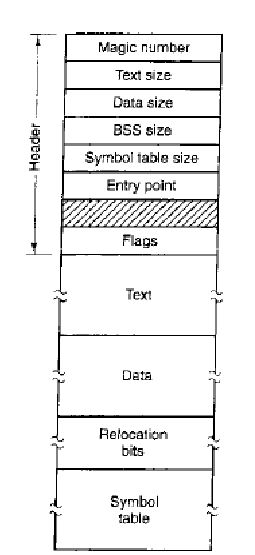
\includegraphics[width=0.2\textwidth]{\imgdir/filesystem_file}
		%\caption{-}
		\label{fig:filesystem_file}
	\end{figure}
	
	For example, whe see a simple executable binary file taken from an early version of UNIX. Although the file is just a sequence of bytes, the operating system will only execute a file if it has the proper format. It has five sectiones: header, text, data, relocation bits, and symbol table. The header starts with a so-called magic number, identifying the file as an executable file (to prevent the accidental execution of a file not in this format). Then comes the sizes of the various pieces of the file, the address at which execution starts, and some flag bits. Following the header are the text and data of the program itself. These are loaded into memory and relocated using relocation bits. The symbol table is used for debugging.

	Having strongly typed files like this causes problems whenever the user does anything that the system designers did not expect.
	
	\item[Acceso de archivo] Tipos de acceso al archivo
	\begin{description}
		\item[Acceso secuencial] A process could read all the bytes or records in a file in order, starting at the beginning, but could not skip around and read them out of order.
		\begin{itemize}
			\item read next
			\item write next
			\item reset
			\item rewrite
		\end{itemize}

		\item[Acceso aleatorio] Can read the bytes or record of a file out of order, or to access records by key rather than by position. Random access files are essential for many applications, like database systems.
		\begin{itemize}
			\item read n
			\item write n
			\item position n
			\begin{itemize}
				\item read next
				\item write next
			\end{itemize}
			\item rewrite n
		\end{itemize}
	\end{description}

	\item[Metadata] Most file systems store the names of all the files in one directory in one place—the directory table for that directory—which is often stored like any other file. Many file systems put only some of the metadata for a file in the directory table, and the rest of the metadata for that file in a completely separate structure, such as the inode.
	\begin{itemize}
		\item Tamaño
		\item Protección
		\item Propietario
		\item Flag hidden
		\item Time stamp (creación, modificación y acceso).
		\item Etc.
	\end{itemize}
\end{description}

\subsubsection{Operaciones sobre archivos}
\begin{itemize}
	\item Create
	\item Delete
	\item Open
	\item Close
	\item Read
	\item Write
	\item Append
	\item Seek
	\item Get attributes
	\item Set Attributes
	\item Rename
\end{itemize}

\subsection{Directorios}
File systems typically have directories (also called folders) which allow the user to group files into separate collections. This may be implemented by associating the file name with an index in a table of contents or an inode in a Unix-like file system. Directory structures may be flat (i.e. linear), or allow hierarchies where directories may contain subdirectories.

\subsubsection{Operaciones sobre directorios}
\begin{itemize}
	\item Create
	\item Delete
	\item Opendir: Abrir un directorio para leer
	\item Closedir
	\item Readdir
	\item Rename
	\item Link: Agregar acceso directo a un archivo
	\item Unlink: Eliminar el acceso directo
\end{itemize}

\subsection{Sistema de archivos}
In computing, a file system (or filesystem) is used to control how data is stored and retrieved. Without a file system, information placed in a storage area would be one large body of data with no way to tell where one piece of information stops and the next begins. By separating the data into individual pieces, and giving each piece a name, the information is easily separated and identified. Taking its name from the way paper-based information systems are named, each group of data is called a ``file''. 

There are many different kinds of file systems. Each one has different structure and logic, properties of speed, flexibility, security, size and more.

Método para guardar y organizar archivos para computadoras y sus datos. Provee acceso y almacenamiento a datos y programas.

Presenta dos aspectos:
\begin{itemize}
	\item Interfaz de usuario: Directorios y Archivos
	\item Implementación.
\end{itemize}

\subsubsection{Partición de discos con MBR}
File systems are stored on disks. Most disks can be divided up into one or more partitions, with independent file systems on each partition. Sector 0 of the disk is called the MBR (Master Boot Record) and is used to boot the computer. The end of the MBR contains the partition table. This table gives the starting and the ending addresses of each partition. One of the partitions in the table is marked as active. When the computer is booted, the BIOS reads in and executes the MBR. The first thing the MBR program does is locate the active partition, read in its first block, called the boot block, and execute it. The program in the boot block loads the operating system contained in that partition. For uniformity, every partition starts with a boot block, even if it does not contain a bootable operating system. Besides, it might contain one in the future.

\begin{figure}[H]
	\centering
	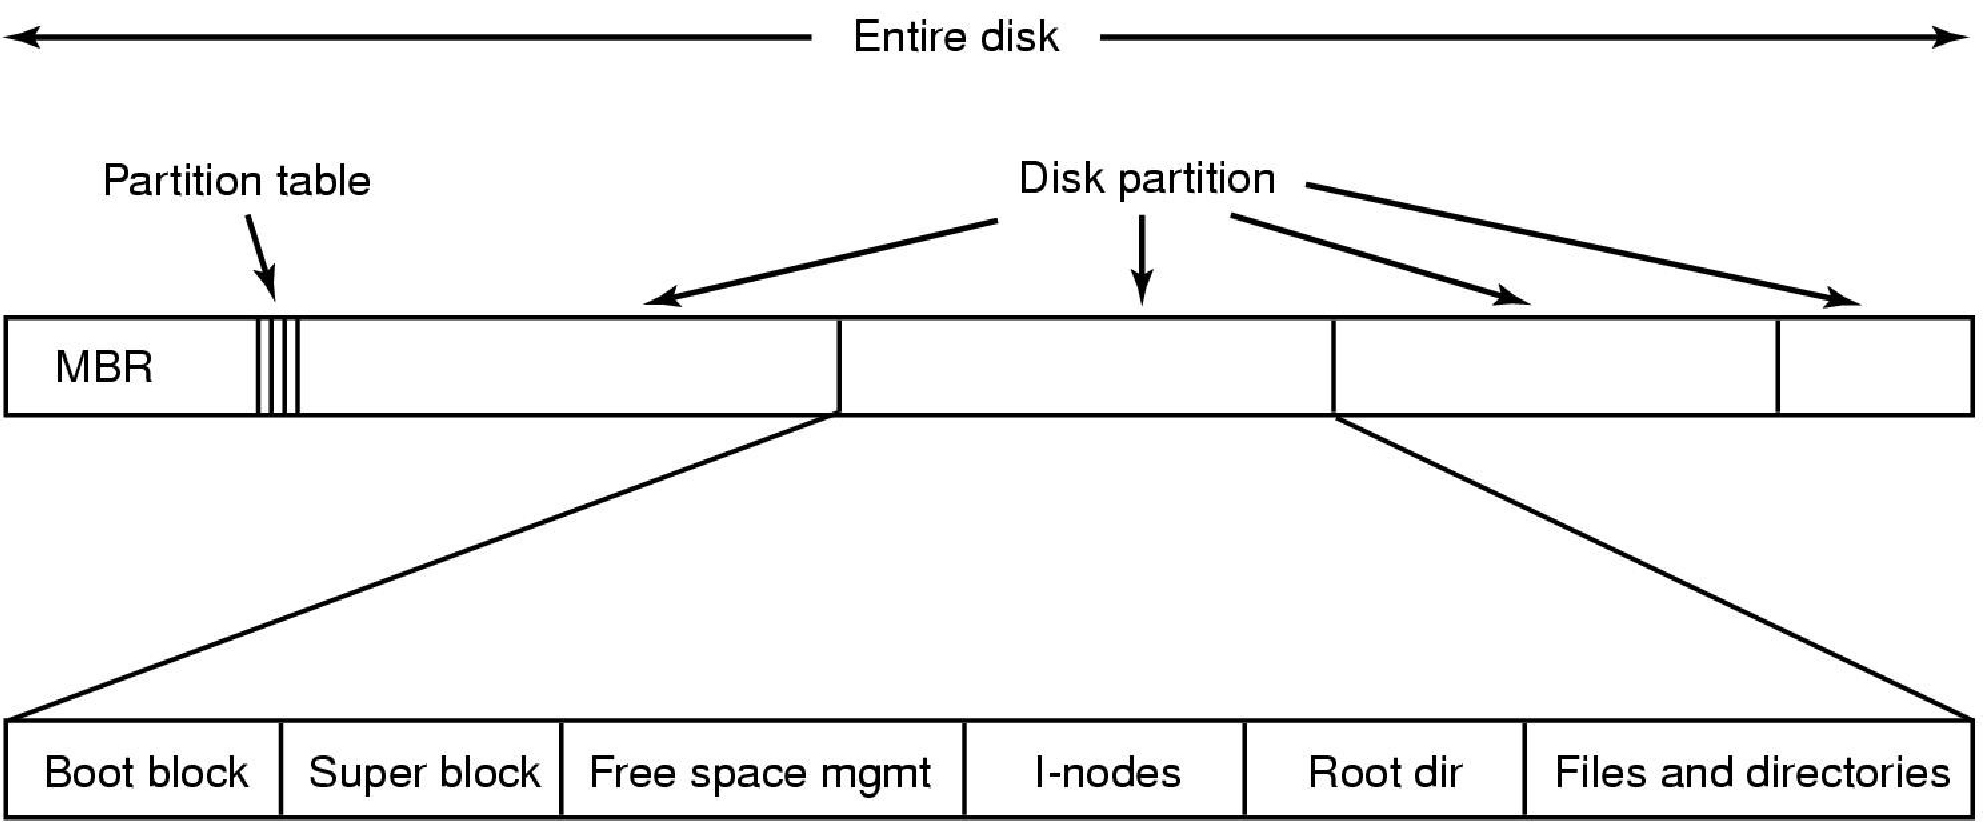
\includegraphics[width=0.6\textwidth]{\imgdir/filesystem_partition_mrb}
	%\caption{-}
	\label{fig:filesystem_partition_mrb}
\end{figure}

Superblock contains all the key parameters about the file system and is read into memory when the computer is booted or the file system is first touched. Typical information in the superblock includes a magic number to identify the file system type, the number of blocks in the file system, and other key administrative information.

Next might come information about free blocks in the file system, for example in the form of a bitmap or a list of pointers. This might be followed by the i-nodes, an array of data structures, one per file, telling all about the file. After that might come the root directory, which contains the top of the file system tree. Finally, the remainder of the disk contains all the other directories and files.

\subsubsection{Particion GUID-EFI}
GUID Partition Table (GPT) is a standard for the layout of the partition table on a physical hard disk, using globally unique identifiers (GUID). Although it forms a part of the Unified Extensible Firmware Interface (UEFI) standard (Unified EFI Forum proposed replacement for the PC BIOS), it is also used on some BIOS systems because of the limitations of master boot record (MBR) partition tables, which use 32 bits for storing logical block addresses (LBA) and size information.

Tiene redundancia.

\subsubsection{Partition table header (LBA 1)}
The partition table header defines the usable blocks on the disk. It also defines the number and size of the partition entries that make up the partition table. The header contains the disk globally unique identifier (GUID). It records its own size and location (always LBA 1!) and the size and location of the secondary GPT header and table (always the last sectors on the disk).

\subsubsection{Paritition entries}
The GPT uses simple and straightforward entries to describe partitions. The first 16 bytes designate the partition type globally unique identifier (GUID). For example, the GUID for an EFI System partition is C12A7328-F81F-11D2-BA4B-00A0C93EC93B. The second 16 bytes contain a GUID unique to the partition. Then follow the starting and ending 64-bit LBAs, partition attributes and partition names. As is the nature and purpose of GUIDs, no central registry is needed to ensure the uniqueness of the GUID partition type designators. The location of the partition entries array on disk is defined in the GPT header.

\begin{figure}[H]
	\centering
	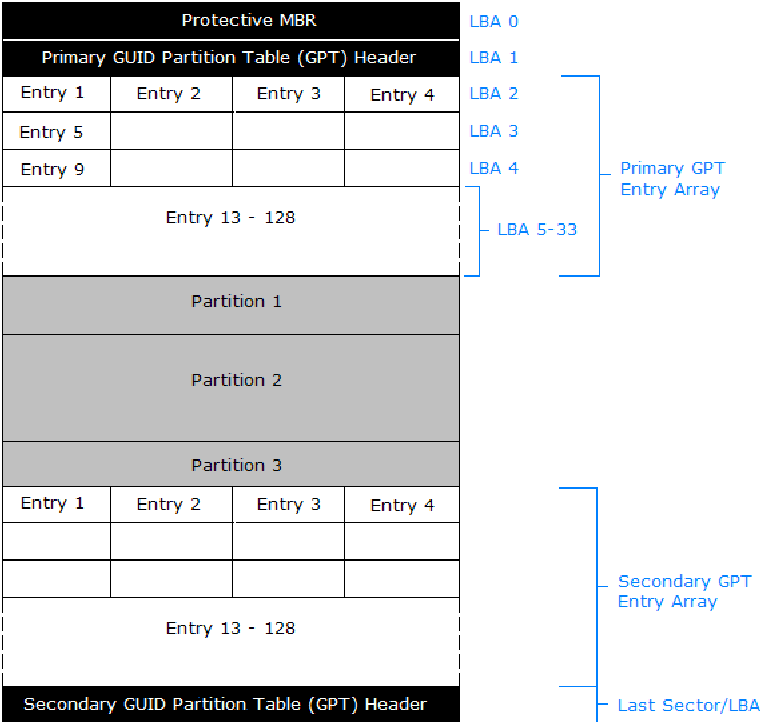
\includegraphics[width=0.6\textwidth]{\imgdir/filesystem_partition_entries}
	%\caption{-}
	\label{fig:filesystem_partition_entries}
\end{figure}

\subsubsection{FAT File System (Linked Allocation)}
File Allocation Table (FAT) is a computer file system architecture and a family of industry-standard file systems utilizing it.

The FAT file system is a legacy file system which is simple and robust. It offers good performance even in light-weight implementations, but cannot deliver the same performance, reliability and scalability as some modern file systems. It is, however, supported for compatibility reasons by nearly all currently developed operating systems for personal computers and many mobile devices and embedded systems, and thus is a well-suited format for data exchange between computers and devices of almost any type and age from 1981 up to the present.

\subsubsection{UNIX File System}
A UNIX directory entry contains one entry for each file in that directory. Each entry is extremely simple because UNIX uses the i-node scheme. A directory entry contains only two fields: the file name and the number of the i-node for that file. 

\begin{figure}[H]
	\centering
	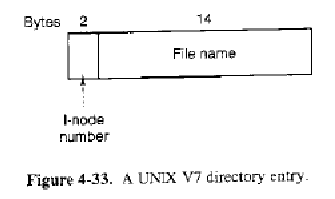
\includegraphics[width=0.4\textwidth]{\imgdir/filesystem_partition_unix_directory_entry}
	%\caption{-}
	\label{fig:filesystem_partition_unix_directory_entry}
\end{figure}

The UNIX i-nodes contain some attributes. The attributes containt the file size, timestamps, owner, group, protection information, and a count of the number of directory entries that pont to the i-node. The latter field is needed due to links. Whenever a new link is made to an i-node, the count in the i-node is increased. When a link is removed, the count is decremented. When it gets to 0, the i-node is reclaimed and the disk blocks are put back in the free list.

\begin{figure}[H]
	\centering
	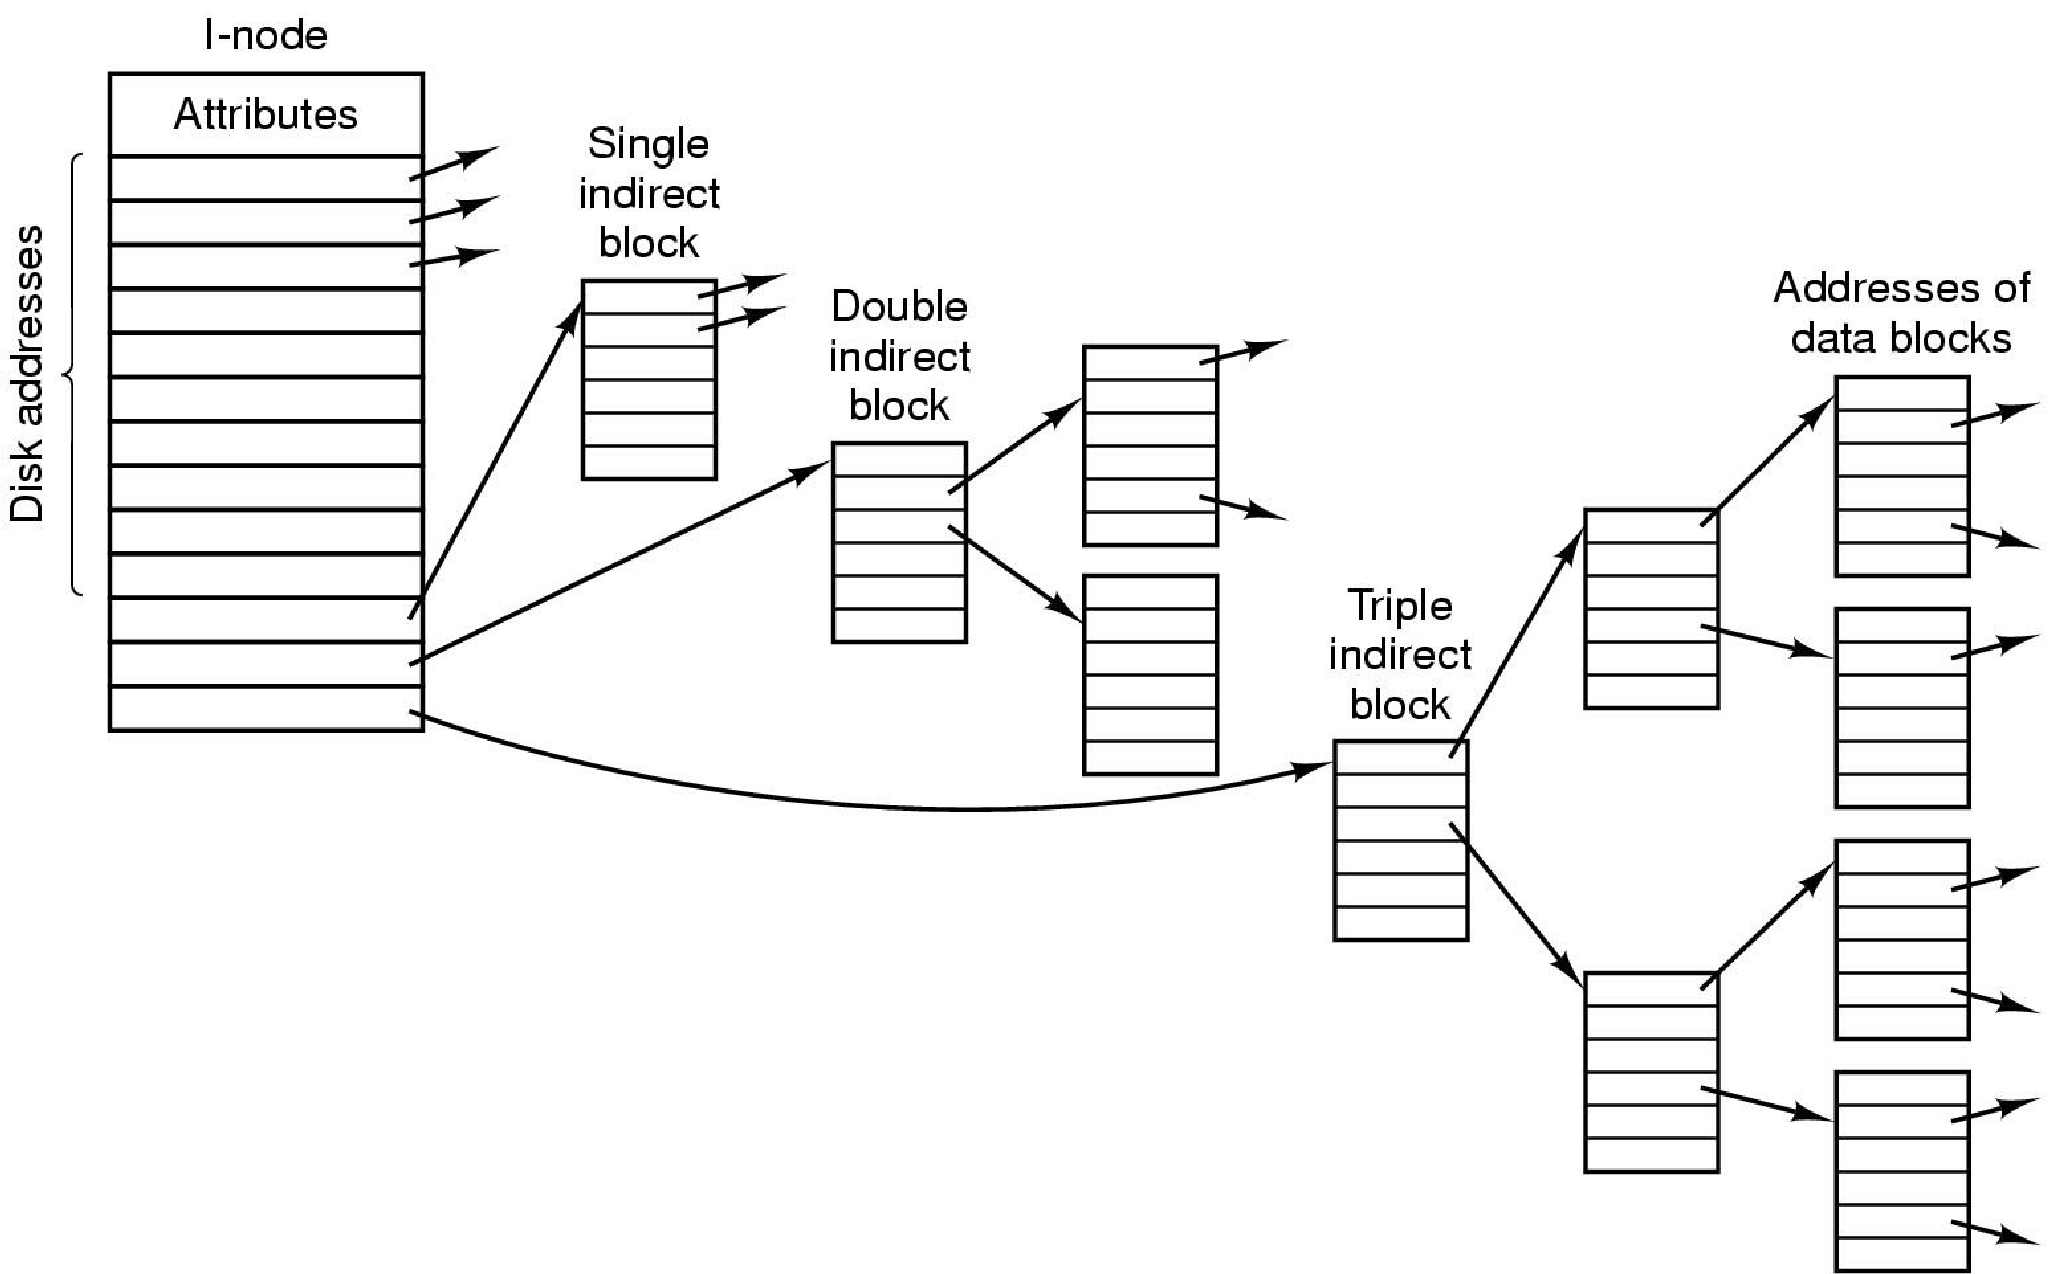
\includegraphics[width=0.6\textwidth]{\imgdir/filesystem_partition_unix_inode}
	%\caption{-}
	\label{fig:filesystem_partition_unix_inode}
\end{figure}

The first 10 disk addresses are stored in the i-node itself, so for small files, all the necessary information is right in the i-node, which is fetched from disk to main memory then the file is opened. For somewhat larger files, one of the addresses in the i-node is the address of a disk block called a single indirect block. This block contains additional disk addresses. If this still is not enough, another address in the i-node, called a double indirect block, contains the address of a block that contains a list of single indirect blocks. Each of these single indirect blocks points to a few hundred data blocks. If even this is not enough, a triple indirect block can be used.

\subsubsection{NTFS (Windows)}
In NTFS, all file, directory and metafile data—file name, creation date, access permissions (by the use of access control lists), and size—are stored as metadata in the Master File Table (MFT). 

A directory entry consists of a filename and a ``file ID'', which is the record number representing the file in the Master File Table. Two copies of the MFT are stored in case of corruption. If the first record is corrupted, NTFS reads the second record to find the MFT mirror file. Locations for both files are stored in the boot sector.

To optimize the storage and reduce the I/O overhead for the very common case of attributes with very small associated value, NTFS prefers to place the value within the attribute itself (if the size of the attribute does not then exceed the maximum size of an MFT record), instead of using the MFT record space to list clusters containing the data; in that case, the attribute will not store the data directly but will just store an allocation map (in the form of data runs) pointing to the actual data stored elsewhere on the volume.

\subsubsection{Transactional NTFS}
Transactional NTFS allows for files and directories to be created, modified, renamed, and deleted atomically. Using transactions ensures correctness of operation; in a series of file operations (done as a transaction), the operation will be committed if all the operations succeed. In case of any failure, the entire operation will rollback and fail. Por ejemplo, ante un corte de energia.

\subsubsection{Log-structured file system}
A log-structured filesystem is a file system in which data and metadata are written sequentially to a circular buffer, called a log.

\subsubsection{Archivos mapeados a memoria}
Api que usa el programador para levantar todo el archivo en memoria (mmap, munmap - map or unmap files or devices into memory).

El archivo queda guardado en un buffer cache en memoria.

The primary benefit of memory mapping a file is increasing I/O performance, especially when used on large files.

Certain application-level memory-mapped file operations also perform better than their physical file counterparts. Applications can access and update data in the file directly and in-place, as opposed to seeking from the start of the file or rewriting the entire edited contents to a temporary location.

A possible benefit of memory-mapped files is a ``lazy loading'', thus using small amounts of RAM even for a very large file. Trying to load the entire contents of a file that is significantly larger than the amount of memory available can cause severe thrashing as the operating system reads from disk into memory and simultaneously writes pages from memory back to disk. Memory-mapping may not only bypass the page file completely, but the system only needs to load the smaller page-sized sections as data is being edited, similarly to demand paging scheme used for programs.

Puede traer:
\begin{itemize}
	\item Problemas de sincronismo
	\item Problemas de performance (manejo de memoria)
\end{itemize}

\subsubsection{Virtual file system}
A virtual file system (VFS) or virtual filesystem switch is an abstraction layer on top of a more concrete file system. The purpose of a VFS is to allow client applications to access different types of concrete file systems in a uniform way. A VFS can, for example, be used to access local and network storage devices transparently without the client application noticing the difference. It can be used to bridge the differences in Windows, Mac OS and Unix filesystems, so that applications can access files on local file systems of those types without having to know what type of file system they are accessing.

A VFS specifies an interface (or a ``contract'') between the kernel and a concrete file system. Therefore, it is easy to add support for new file system types to the kernel simply by fulfilling the contract.

\begin{figure}[H]
	\centering
	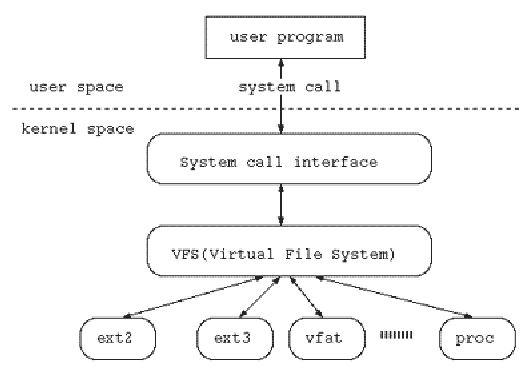
\includegraphics[width=0.6\textwidth]{\imgdir/filesystem_partition_vfs}
	%\caption{-}
	\label{fig:filesystem_partition_vfs}
\end{figure}

Interactúa con los File Systems, que interactúan con el buffer cache, el pagecache y los dispositivos.

Interactúa con el usuario por medio de las System Calls.

\newpage
\section{Clustered file systems}
Es un file system que va ser accedido simultáneamente desde más de un cliente.

En general NO es usado por los clusters.

Proveen un mecanismo de control de concurrencia y de serialización.

\subsection{RAID: Redundant Array of (Inexpensive/ Independent) Disks}
RAID (originally redundant array of inexpensive disks; now commonly redundant array of independent disks) is a data storage virtualization technology that combines multiple disk drive components into a logical unit for the purposes of data redundancy or performance improvement.

Data is distributed across the drives in one of several ways, referred to as RAID levels, depending on the specific level of redundancy and performance required. The different schemes or architectures are named by the word RAID followed by a number (e.g. RAID 0, RAID 1). Each scheme provides a different balance between the key goals: reliability, availability, performance, and capacity. RAID levels greater than RAID 0 provide protection against unrecoverable (sector) read errors, as well as whole disk failure.

Hoy es un término ``paraguas'' para replicar y dividir datos entre varios discos. Pero vistos como un solo disco por el Sistema Operativo.


\subsubsection{Principios del RAID}
Combinar varios discos físicos en una única unidad lógica por Software o Hardware

Para lograr estos objetivos utiliza los conceptos de Mirror o redundancia de datos, Stripping o distribución de bloques de datos y Corrección de errores.

\begin{description}
	\item[Data Stripping o Distribución de Bloques de datos] Es la técnica de segmentar datos secuencialmente lógicos, como un archivo, de manera que segmentos consecutivos son almacenados en dispositivos de almacenamiento distintos. Este mecanismo es útil cuando un proceso que accede a un dispositivo necesita acceso a datos de manera más veloz de la que este dispositivo puede proveer. Permite acceder a los datos de manera concurrente.

	\item[Disk mirroring o Redundancia de Datos] Es la replicación de volúmenes de discos en discos duros separados para asegurar la disponibilidad continua. La replicación se realiza a través de microcódigo en el controlador del disco o mediante software de servidor. Sirve como copia de seguridad de los datos ante alguna falla de hardware.

	\item[Error detection and correction o Corrección de errors] Son técnicas que permiten tener datos seguros de información digitalizada a través de canales de comunicación inseguros. Se basa en utilizar bits de paridad para detector fallas en los datos.
\end{description}

\subsubsection{Niveles de RAID}
\begin{description}
	\item[RAID 0] \emph{A RAID 0 (also known as a stripe set or striped volume) splits data evenly across two or more disks (striped)}, without parity information and with speed as the intended goal. RAID 0 was not one of the original RAID levels and provides no data redundancy. RAID 0 is normally used to increase performance, although it can also be used as a way to create a large logical disk out of two or more physical ones.
	\begin{figure}[H]
		\centering
		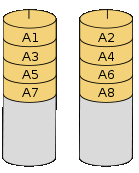
\includegraphics[width=0.15\textwidth]{\imgdir/clustered_filesystem_raid_0}
		%\caption{-}
		\label{fig:clustered_filesystem_raid_0}
	\end{figure}
	Accessing the stripes in the order A1, A2, A3, ... provides the illusion of a larger and faster drive.

	\item[RAID 1] \emph{An exact copy (or mirror) of a set of data on two disks}. This is useful when read performance or reliability is more important than data storage capacity. Such an array can only be as big as the smallest member disk. A classic RAID 1 mirrored pair contains two disks.
	\begin{figure}[H]
		\centering
		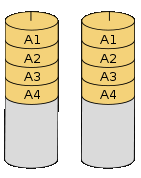
\includegraphics[width=0.15\textwidth]{\imgdir/clustered_filesystem_raid_1}
		%\caption{-}
		\label{fig:clustered_filesystem_raid_1}
	\end{figure}

	\item[RAID 2] A RAID 2 stripes data at the bit (rather than block) level, and uses a Hamming code for error correction. All hard disks eventually implemented Hamming code error correction. This made RAID 2 error correction redundant and unnecessarily complex. This level quickly became useless and is now obsolete. There are no commercial applications of RAID 2.

	\item[RAID 3] Byte stripping con disco de paridad (para detectar si hubo errores).

	\item[RAID 4] Block-level striping with a dedicated parity disk. A block, sometimes called a physical record, is a sequence of bytes or bits, usually containing some whole number of records.
	\begin{figure}[H]
		\centering
		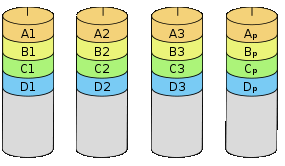
\includegraphics[width=0.3\textwidth]{\imgdir/clustered_filesystem_raid_4}
		%\caption{-}
		\label{fig:clustered_filesystem_raid_4}
	\end{figure}

	\item[RAID 5] A RAID 5 comprises block-level striping with distributed parity. Unlike in RAID 4, parity information is distributed among the drives. RAID 5 requires at least three disks.
	\begin{figure}[H]
		\centering
		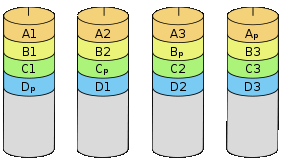
\includegraphics[width=0.3\textwidth]{\imgdir/clustered_filesystem_raid_5}
		%\caption{-}
		\label{fig:clustered_filesystem_raid_5}
	\end{figure}

	\item[RAID 6] Block Stripping con doble paridad distribuida.

	\item[RAID anidados] Levels of nested RAID, also known as hybrid RAID, combine two or more of the standard levels of RAID (redundant array of independent disks) to gain performance, additional redundancy, or both. Muchos de estos niveles están en software.
	\begin{figure}[H]
		\centering
		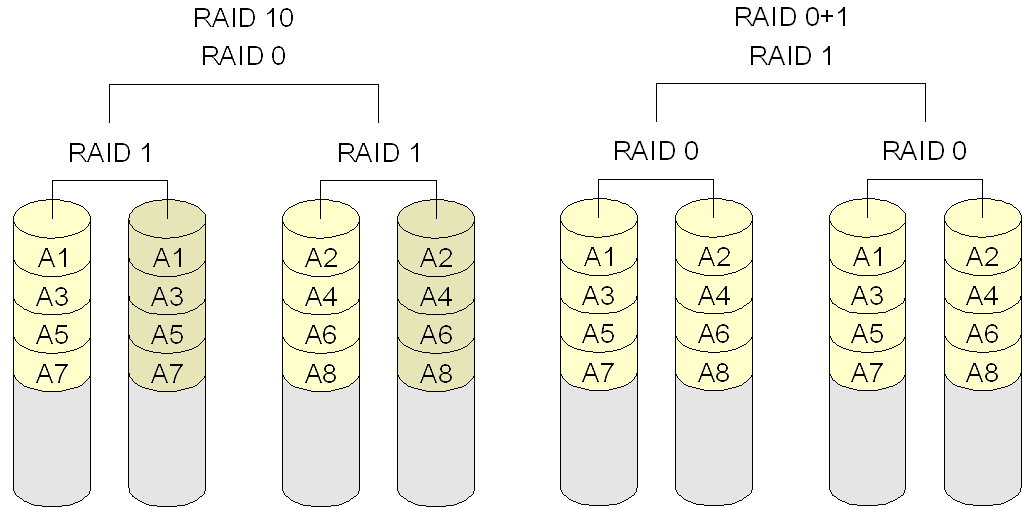
\includegraphics[width=0.45\textwidth]{\imgdir/clustered_filesystem_raid_hybrid}
		%\caption{-}
		\label{fig:clustered_filesystem_raid_hybrid}
	\end{figure}
\end{description}

\subsubsection{Software RAID vs. Hardware RAID}
\begin{description}
	\item[Software RAID] El procesador debe usar su tiempo para las operaciones de RAID en una capa entre el File System y el Device Driver.

	\item[Hardware RAID] Requiere un controlador dedicado. Este controlador dedicado es un dispositivo que maneja los discos físicos y los presenta al computador como unidades lógicas. Dado que eventualmente este controlador implementa hardware RAID es llamado frecuentemente controlador RAID. Además provee cache adicional.

	Un disk array controller debe proveer interfaces fron-end hacia los disco y back-end hacia el host.

	A disk array controller provides front-end interfaces and back-end interfaces.
	\begin{itemize}
		\item Back-end interface communicates with controlled disks. Hence protocol is usually ATA (a.k.a. PATA; incorrectly called IDE), SATA, SCSI, FC or SAS.
		\item Front-end interface communicates with a computer's host adapter (HBA, Host Bus Adapter)
	\end{itemize}

	\item[Fake RAID] Es un controlador de firmware que toma las funciones de raid durante el boot. Una vez que el kernel de un SO está cargado, el control pasa al SO.

	Esto se debe a que Windows no puede bootear de software RAID y por lo tanto durante el boot delega esta tarea en el controlador de firmware. 

	Se trata de un software RAID que carga al procesador con un  controlador de múltiples canales ATA.
\end{description}

\subsection{NAS (Network Attached Storage)}
Network Attached Storage conecta un file-sytem remoto a una red, proveyendo el acceso a clientes heterogéneos. NAS aparece ante un sistema operativo cliente como un servidor.

NAS devices began gaining popularity as a convenient method of sharing files among multiple computers. Potential benefits of dedicated network-attached storage, compared to general-purpose servers also serving files, include faster data access, easier administration, and simple configuration. Provee servicios basados en archivos.\\

Generalmente es una versión reducida empotrada de algún Sistema Operativo.

NAS is useful for more than just general centralized storage provided to client computers in environments with large amounts of data. NAS can enable simpler and lower cost systems such as load-balancing and fault-tolerant email and web server systems by providing storage services.

\subsection{SAN (Storage Area Network)}
Storage Area Network conecta dispositivos remotos que el SO ve como locales (e implementa el file system).
One way to loosely conceptualize the difference between a NAS and a SAN is that NAS appears to the client OS (operating system) as a file server (the client can map network drives to shares on that server) whereas a disk available through a SAN still appears to the client OS as a disk, visible in disk and volume management utilities (along with client's local disks), and available to be formatted with a file system and mounted. SAN no provee la abstracción de archivos, solo operaciones en bloques.

Consolida las ``islas de discos'' con conexiones de red.

Pueden ser discos o RAIDs o alguna arquitectura no RAID

Requieren de un software de administración.

Algunas proveen capacidades RAID.

\begin{figure}[H]
	\centering
	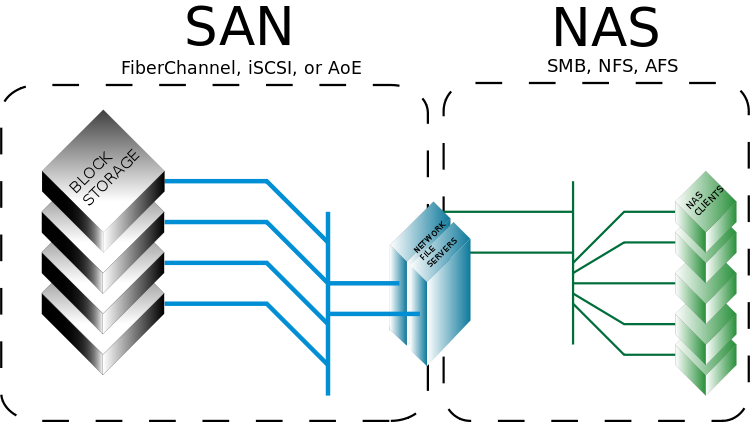
\includegraphics[width=0.45\textwidth]{\imgdir/clustered_filesystem_san_nas}
	%\caption{-}
	\label{fig:clustered_filesystem_san_nas}
\end{figure}

\newpage
\section{Móviles}
\subsection{Sistemas operativos en móviles}
Usuarios están poco tiempo en varias aplicaciones (Con interacciones cortas).

Lanzamiento y conmutación (switching) rápida entre apps. (200 ms)

Simplificar el uso de las apps (lanzamiento, cierre, inter-operación)

Neutralidad del diseño del Sistema Operativo: el diseño te fuerza solo al look \& feel (siempre que no comprometa al SO).

\subsection{Android}
Usó hasta la versión 4.4.3 una JVM llamada Dalvik basada en Apache Harmony. Dalvik es una JVM más reducida que la JVM común.

Programs are commonly written in Java and compiled to bytecode for the Java virtual machine, which is then translated to Dalvik bytecode and stored in .dex (Dalvik EXecutable) and .odex (Optimized Dalvik EXecutable) files; related terms odex and de-odex are associated with respective bytecode conversions. The compact Dalvik Executable format is designed for systems that are constrained in terms of memory and processor speed.

Desde Lolipop usa Android Runtime.

\subsubsection{Arquitectura}
\begin{figure}[H]
	\centering
	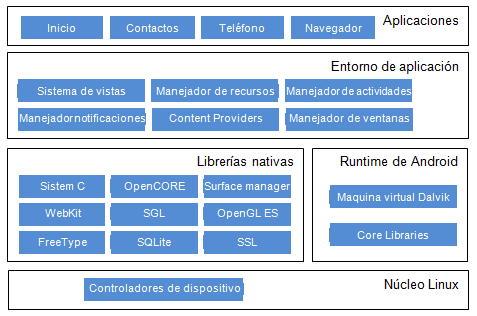
\includegraphics[width=0.7\textwidth]{\imgdir/android_arquitectura}
	%\caption{-}
	\label{fig:android_arquitectura}
\end{figure}

\subsubsection{Android Run Time (ART)}
Compila al instalar la aplicación. AOT (Ahead of Time) Compilation.
\begin{itemize}
	\item Mejora el tiempo de respuesta y la vida de la batería
	\item Aunque el código AOT no es mas rápido que el JIT (Just in Time).
	\item Y se pierden aspectos dinámicos
\end{itemize}
Transforma DEX en ELF

\subsubsection{Aplicaciones}
Las aplicaciones vienen empaquetadas en un archivo .apk. Una vez instalada tiene su sandbox, cada apk es un usuario de linux con permisos y directorio propios.

Cada aplicación corre en su propio proceso con su propia copia de Dalvik. Los procesos son provistos por el kernel y manejados por el Android Run Time. Para mantener la respuesta del sistema, el sistema Android puede matar sin aviso a procesos que considera que no están respondiendo (y las aplicaciones contenidas dentro del mismo).

Los componentes están descriptos en un Manifest (XML).

Hay mecanismos para compartir datos entre distintas aplicaciones.

Hay una previsión para notificaciones asincrónicas

\subsubsection{Activity}
Una activity es una aplicación que se comunica por medio de una pantalla con el usuario. Generalmente, esta comunicación se realiza fullscreen, pero puede ser una pantalla flotante. Una aplicación está compuesta por una o más activities, pero sólo una puede estar activa a la vez. El resto de las activities se guarda en un stack.

\begin{description}
	\item[Ciclo de vida] ~
	\begin{description}
		\item[Active] está al tope del stack e interactuando con el usuario.
		\item [Paused] visible pero sin foco.
		\item [Stopped] queda en memoria pero ya terminó. Candidata al kill.
		\item [Inactive] fuera de la memoria. Debe lanzarse nuevamente.
	\end{description}		
\end{description}

\begin{figure}[H]
	\centering
	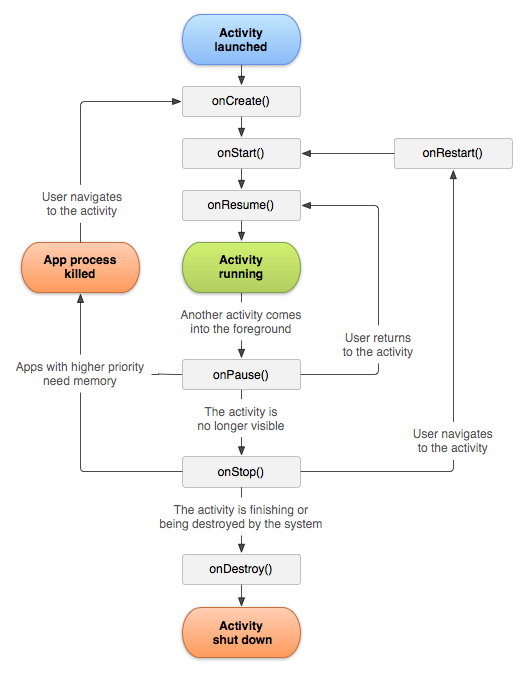
\includegraphics[width=0.6\textwidth]{\imgdir/android_activity_lifecycle}
	%\caption{-}
	\label{fig:android_activity_lifecycle}
\end{figure}

\subsubsection{Zygote}
Zygote is a daemon which only mission is to launch applications. This means that Zygote is the parent of all App process. When app\_process launches Zygote, it creates the first Dalvik VM and calls Zygote's \texttt{main()} method. Once Zygote starts, it preloads all necessary Java classes and resources, starts System Server and opens a socket \texttt{/dev/socket/zygote} to listen for requests for starting applications. 

Zygote receives a request to launch an App through \texttt{/dev/socket/zygote}. Once it happens it trigger a \texttt{fork()} call. Here is where the virtues of a great design take action. When a process forks, it creates a clone of itself. It replicates itself in another memory space. This is done pretty efficiently. When this happens to Zygote, it creates an exact and clean new Dalvik VM, preloaded with all necessary classes and resources that any App will need. This makes the process of creating a VM and load resources pretty efficiently. But the design goes farther. As we know, Android runs on Linux. The Linux Kernel implements a strategy call Copy On Write (COW). What this means is that during the fork process, no memory is actually copy to another space. It is shared and marked as copy-on-write. Which means that when a process attempt to modify that memory, the kernel will intercept the call and do the copy of that piece of memory. In the case of Android those libraries are not writable. This means that all process forked from Zygote are using the exact same copy of the system classes and resources. 

Another benefit is the real memory saving. No matter how many applications are started the increase in memory usage will be a lot smaller.

\subsubsection{Wake locks}
El hardware de Android pasa a sleep apenas queda ocioso. Si se necesita mantener a la CPU activa se pueden usar Wake Locks. Los Wake Locks sirven para que la aplicación quede activa, a costa de gastar la batería.

\subsection{Apple IOS}
Sistema operativo de iPhone, iPod touch, Apple TV e iPad.

Basado en Darwin.

Objective-C como lenguaje preferido.

\subsubsection{Kernel}
\textbf{Usa un Kernel híbrido}

The idea behind a hybrid kernel is to have a kernel structure similar to that of a microkernel, but to implement that structure in the manner of a monolithic kernel. In contrast to a microkernel, all (or nearly all) operating system services in a hybrid kernel are still in kernel space. So there are none of the reliability benefits of having services in user space, as with a microkernel. However, just as with an ordinary monolithic kernel, there is none of the performance overhead for message passing and context switching between kernel and user mode that normally comes with a microkernel. Pasaje de mensajes y protección de memoria.

\begin{figure}[H]
	\centering
	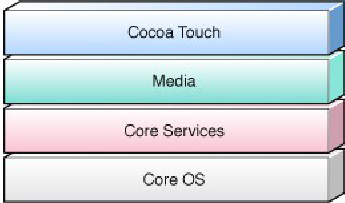
\includegraphics[width=0.35\textwidth]{\imgdir/ios_capas_abstraccion}
	\caption{Las 4 capas de abstracción de IOS}
	\label{fig:ios_capas_abstraccion}
\end{figure}

\subsubsection{Cocoa Touch}
Es el framework para el desarrollo de aplicaciones
\begin{itemize}
	\item Auto-Layout y StoryBoards
	\item Multitasking y Printing
	\item Data Protection (encriptado)
	\item Push y Local Notifications
	\item UIState Preservation
	\item Reconocimiento de gestos y display externo
	\item MVC standards
\end{itemize}

\begin{description}
	\item[Media Layer] Manejo de Audio, Video y Gráficos.

	\item[Core Services Layer] ~
	\begin{itemize}
		\item Servicios fundamentales usados por las aplicaciones: iCloud, Bloqueo de Objetos, Grand Central Dispatch, SQLite, XML, InAppPurchase
		\item Core Frameworks: Foundation, AddressBook, Location, TE, Eventos, Store
	\end{itemize}

	\item[Core OS Layer] Frameworks de bajo nivel
	\begin{itemize}
		\item Accelerate (math,DSP, vector)
		\item External Accesories (hardware externo)
		\item Security
		\item System: Threading (POSIX threads), Networking (BSD sockets), File-system access, Standard I/O, Bonjour and DNS services, Locale information, Memory allocation
	\end{itemize}
\end{description}

\subsubsection{Procesos}
\textbf{Corren bajo dos UIDs, root (0), algunos del sistema y mobile (501).}

\textbf{Todos los procesos tienen la misma UID, pero no se comunican directamente.}

No se pueden manejar en forma directa.

Al pasar a background provocan un evento y quedan suspendidos.

Pueden cerrarse usando la taskbar.

\subsubsection{iCloud}
Sincroniza los datos del usuario en todos los dispositivos asociados a la cuenta de iCloud.

Usa Ubiquity Containers, se guardan:
\begin{itemize}
	\item Key-Value files 
	\item Document Files
	\item Core-Data Files
\end{itemize}

To save data to iCloud, your app places data in special file system locations known as iCloud containers. An iCloud container (also referred to as a ubiquity container) serves as the local representation of the corresponding iCloud storage. It is separate from the rest of your app's data. 

\begin{figure}[H]
	\centering
	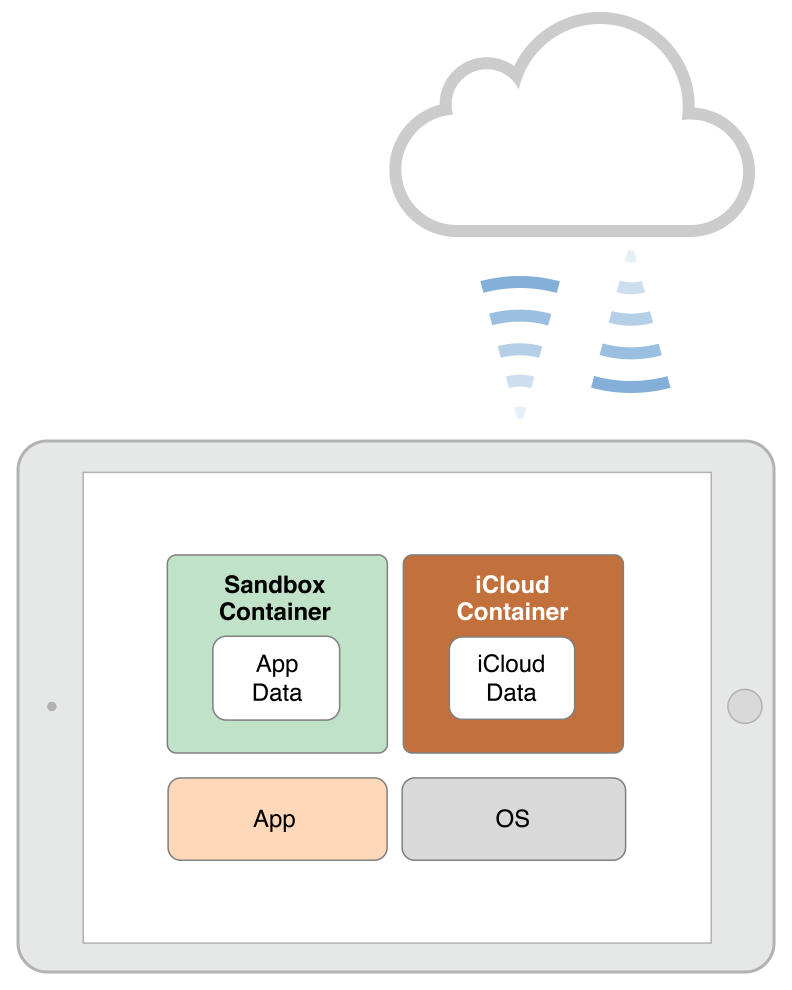
\includegraphics[width=0.35\textwidth]{\imgdir/ios_icloud}
	%\caption{-}
	\label{fig:ios_icloud}
\end{figure}

\subsubsection{Procesos y Tasks en XNU}
Un proceso BSD tiene al menos una task.

Las tasks indican una unidad ejecutable en su ambiente de ejecución (flavor). Puede haber tasks sin procesos BSD asociados.

Los threads son las unidades de ejecución.

\subsubsection{Concurrencia GCD}
Permite que las tasks corran en paralelo encolándolas y planificándolas (``routing'').

Maneja la concurrencia usando Dispatch Queues.

\subsubsection{Threads}
Apple trata que no se usen threads en forma directa.

Cada thread tiene un run-loop para manejar eventos. Un run-loop tiene un ``modo'' que indica que eventos recibe.

\subsubsection{Grand Central Dispatch}
Tecnología para soportar multiprocesamiento simétrico. Es una implementación del patrón thread-pool. Semaforo para los threads.

% Bibliografía utilizada en el apunte
\newpage
\newcommand{\bibliographyname}{Bibliografía} % Defino el nombre de la sección de la bibliografía
\addcontentsline{toc}{section}{\bibliographyname} % Agrego la bibliografía en el índice
\renewcommand\refname{\bibliographyname} % Renombro a la bibliografía (por default es 'Referencias')
\begin{thebibliography}{X}
	\bibitem{tanenbaum} \textsc{Andrew S. Tanenbaum}, \textit{Sistemas Operativos Modernos}, tercera edición, PEARSON EDUCACIÓN, México, 2009.
\end{thebibliography}

% Incluir los nombres de las personas que han colaborado en la creación del apunte
\colaborador{Kaoru Heanna}
\colaborador{Darío Miñones}
\colaborador{Matías Lafroce}
\colaborador{Ezequiel Pérez Dittler}
%\revisor{Dr. Profesor}{10/01/2015}
\makeseccioncolaboradores % Crea la sección de colaboradores

% Incluir el historial de cambios
\revision{21/02/2015}{Versión inicial con las secciones de Introducción y de Mecanismos básicos.}
\revision{22/02/2015}{Se agregó la sección de Procesos y de Threads.}
\revision{23/02/2015}{Se agregó la sección de Administración de memoria y de Memoria virtual.}
\revision{28/02/2015}{Se agregó la sección de Linker y de Bibliotecas.}
\revision{08/03/2015}{Se agregó la sección de Virtualización.}
\revision{09/03/2015}{Se agregó la sección de Sistemas de archivos y Clustered filesystem.}
\revision{10/03/2015}{Se agregó la sección de Móviles.}
\makehistorial

\end{document}
